\documentclass[12pt, twoside]{book}

%Languages
\usepackage[T2A]{fontenc}
\usepackage[utf8]{inputenc}
\usepackage[english, russian]{babel} 

\usepackage{textbook}

\author{Гущин Д. Д.}
\title{Теория графов}
\date{\today}

\begin{document}
    \maketitle
    \tableofcontents
	\sloppy
\chapter*{От автора}
\addcontentsline{toc}{chapter}{От автора}

\epigraph{\itshape Они слили вместе религию, искусство и науку: 
ведь наука в конечном счете --- исследование чуда, коего мы не в силах объяснить,
а искусство~---~толкование этого чуда.}{--- Рэй Брэдбери, \textit{Марсианские хроники}}

	Во время длительного процесса редактирования книги я преследовал постоянно цель 
	уберечь читателя от траты времени на те факты, с которыми он уже знаком, добавляя для этого много сопутствующих примечаний. 
	Из-за этого некоторые части пособия раздувались так, что хотелось взять метлу с совком и выгрести весь мусор из них. 
	
	Поэтому я решил еще до начала пособия предупредить читателя: если во время чтения пособия 
	вы видите знакомый вам материал, не стоит тратить на него много времени, а, вероятно, стоит даже пропустить его. 
	Этот же совет касается тех разделов, которые будут вызывать у вас мигрени, желание~---~пойти отдохнуть. 
	Следуя этому совету, вы сможете, как на ковре-самолете, пролететь над теорией графов и алгоритмов, 
	<<насладится видами>> и не влететь на скорости в непреодолимые для вас <<стены>>.
	
	Первая глава наполнена материалом, необходимым для новичков и всем тем, 
	кому нравится не только изучать математику, но и обозревать истории, возникающие в процессе становления этой науки.
	
	Вторая глава была создана в помощь мне для проведения курса теории графов в <<Phystech.International $2018$>> 
	и в течение этого лагеря эволюционировала, приобретая много нового, что я почерпнул из общения со школьниками.
	Вот список тех, кто первым прослушал этот курс: Саморуков М. А., Прокопец П. А., Верещагина С. В., Шиндян Д. С.,
	Троян-Головян В. Д., Михеева Т. А., Кушнир А. В., Волгина Е. К.
	
	Третья глава получена дополнением второй главы до целостного курса графов, который рассказывается в некоторых ВУЗах.
	В первую очередь, использовался материал из одноименных книг А. В. Омельченко и Ф. Харари по теории графов. Кроме того,
	автор почерпнул очень много интересных фактов из курса <<Дискретных структур>>, читавшегося на ФИВТе МФТИ в $3$-ем 
	семестре и составленного прекрасным преподавателем А. Дайняком.
	
	Четвертая глава пока что находится на очень ранней стадии разработки и предварительно она будет содержать материал, 
	собранный мной в процессе прослушивания курса алгоритмов на $1$ курсе ФУПМа МФТИ.
	
	\emph{Sapere Aude!} (Дерзайте знать!)

\begin{flushright}
\textit{Дима Г.}

\textit{\today}
\end{flushright}
	\sloppy
\chapter{Элементы теории графов}
\section{О том, как появилась теория графов...}

\mysubsection{История развития}
	Путь, по которому развивается любая область математики можно сравнить с русскими дорогами: то там, то здесь встретится выбоина, в которую если попадешь, то выбраться сможешь не скоро. Под этими <<выбоинами>> можно понимать великие математические загадки: формулировки у них простые, а вот доказательства~---~нет.
	
	Неоднократны случаи, когда математические задачи искали своего решения не одно столетие, а некоторые из них до сих пор его и не нашли. Стоит только вспомнить нашумевшую в конце XX века Великую теорему Ферма, которую всё-таки смог в $1994$ году доказать Эндрю Уайлс. Однако, как показала практика, между доказанной и недоказанной теоремой мало отличий, с практической точки зрения, а значит, и пользы должны быть мало от этого. Так, почему же за их решение часто дают престижные премии и так почитают математиков, которые смогли одолеть эти задачи?
	
	Дело в том, что какая-то задача становится великой в тот момент, когда существующего математического аппарата не хватает для её решения. В этом ключе великие задачи похожи на высокие крепостные стены, которые видны из далека и до которых путь не близок. И преодолевая этот путь, исследователи совершенствуют свой рабочий инструмент, открывая удивительные возможности математики. Именно по такому пути и начала своё развитие теория графов.

	Достоверно известно, что впервые эта теория была затронута в одной из работ Леонарда Эйлера, опубликованной в $1736$ году. В ней Эйлер сформулировал и решил <<Задачу о семи кёнигсбергских мостах>>. Как и всегда, математические головоломки использовались скорее в качестве развлечения и не предвещали новые открытия, поэтому долгое время теория графов не имела широкого применения и не воспринималась всерьёз.  

	Однако некоторые всё-таки преуспели в этом деле. Так, например, в $1852$ году Фрэнсисом Гутри была сформулирована гипотеза о четырёх красках. Понадобилось почти $120$ лет, чтобы решить её. Позже мы ещё вернемся к ней и обсудим преграды, которые возникли на пути математиков в процессе решения этой задачи.
	
	В XIX веке произошёл значительный скачок в теории графов, связанный с развитием теории электрических цепей и органической химии. В~$1847$ году Густав Кирхгов доказал матричную теорему о деревьях, а в~$1889$ году Артур Кэли, английский математик, доказал одноименную теорему о числе остовных деревьев полного графа. С начала $30$-х годов XIX века математики, как голодные звери, постепенно стягивались на эту сладкую и новую область, в которой, как оказалось, далеко не всё было очевидным.
	
	Несмотря на бурное развитие этой теории, до XX века она представляла из себя очень разрозненные области, которые имели общим началом только сам граф. С середины XX века появились успешные попытки структуризовать её: в частности, в этом деле преуспели К. Берж, О. Оре, Ф. Харари. Ещё один рывок в этом направлении был сделан совсем недавно, около 30 лет назад, Тимом Бернерс-Ли, который создал Интернет. Впоследствии, как мы знаем, Всемирная паутина обрела невероятные масштабы и теперь все передачи, шифрование основано на алгоритмах на графах.
	
	Благодаря элегантному, стройному виду, в который облачили теорию графов математики середины и конца XX века, её начали активно использовать при составлении олимпиад для школьников и студентов, включили во многие студенческие программы. Такая практика только укрепила фундамент этой теории и дала толчок к появлению большого числа методических пособий, направленных на неподготовленного читателя. До сих пор скорость развития теории графов не снизилась и всё большее число математиков устремляют свой взгляд в сторону графов.
\begin{paracol}{2}
	Как мы только что поняли, в становлении теории графов большую роль сыграла практика. Как именно? Когда специалист сталкивался с какими-то операциями, связями, отношениями, он пытался их изобразить в качестве рисунка. При этом суть самих вещей опускалась, то есть было не важно, как изобразить объект, поэтому было удобно для этого на рисунке поставить просто точку.
	
	Далее надо было указать отношения между этими точками и вполне логично было соединять точки линиями. В некоторых ситуациях, чтобы указать отличительную особенность отношений между объектами, стоило рисовать вместо линии стрелку.
	
	Таким образом, и начали появлятся графы~---~рисунки с вершинами, некоторые из которых соединены линиями.
	 
\switchcolumn

\begin{tikzpicture}
	\path (144:1.5) edge [bend right=45](216:1.5)
    	  (144:1.5) edge [bend left=30] (288:1.5);	
   	 
	\Loop [dist=2cm, dir=EA](0:1.5);
	\Loop [dist=2cm, dir=NO](72:1.5);
	\Loop [dist=2cm, dir=NOWE](144:1.5);
	\Loop [dist=2cm, dir=SOWE](216:1.5);
	\Loop [dist=2cm, dir=SOEA](288:1.5);
	
	\Loop [dist=2cm, dir=NO](260:5);  
	
	\tikzstyle{every node}=[circle, draw, fill=red, inner sep=0pt, minimum width=6pt]
	
	\foreach \x in {0,72,...,288}
    {
    	\draw [->, >=stealth']
    	(\x:1.5) node {} -- (\x+72:1.5)
    	(\x:1.5) node {} -- (\x+144:1.5)
    	(\x:1.5) node {} -- (\x+216:1.5)
    	(\x:1.5) node {} -- (\x+288:1.5);
    };
    
    \draw (255:2.5) node {} -- (285:4.5) node {} -- (265:6) node {} -- (260:5) node {};
      
    
    \draw \foreach \x in {0,72,...,288}
    {
    	(\x:1.5) node {}
    };
\end{tikzpicture}\begin{center}
	Рис. 1. Абсолютно произвольный граф 
\end{center}\end{paracol}
	
	После того, как задача формулировалась на языке теории графов, математики указывали параметры, которые были весомыми в рамках поставленной задачи. Так, в каких-то задачах надо было изображать ориентированные графы, в других~---~планарные, в тех, которые были связаны с сетями,~---~взвешенные, случайные. С помощью расширения области применения графов вариативность графов расширялась, открывая невероятные миры перед математиком.	 

	Математики отвечали взаимностью на такое разнообразие графов: у них появлялось невероятное число вопросов, на которые должна была ответить теория графов. Смешение возможностей этой новой области и рвения самых любопытных математиков привело к тому, что графы заняли одно из самых главных мест в комбинаторике. 
	
	Мать теории графов~---~комбинаторика~---~начала своё существование более двух тысячелетий назад, хотя сам термин был введён только в $1666$ году Лейбницем. Этот раздел математики сильно расширил свои владения, завладев частью теорий экстремальных задач, топологии, теории вероятностей. Кроме такой экспансии, она породила ещё несколько своих направлений: теорию графов, теорию Рамсея, перечислительную комбинаторику. Последуем же в след названию этой книги и окунёмся в мир теоретико-графовых моделей!
	
\mysubsection{Примеры}	
	
	Разберём два примера, которые можно отнести к самому нижнему ярусу школьной олимпиадной математики. Они покажут нам, как с помощью несложных рассуждений в рамках теории графов можно буквально разломить задачу и достать искомый ответ.
	
	Оба примера позаимствованы из книги <<Ленинградские математические кружки>>, в которой любознательный читатель может найти много схожих интересных задач. В этой книге также увлекательно изложены многие темы, которые было бы полезно освоить начинающему олимпиаднику.
\begin{example}
	Между $9$-ю городами России введены участки высокоскоростной автомагистрали. Есть следующие марщруты: Москва~---~Казань, Владивосток~---~Архангельск, Москва~---~Владивосток, Владивосток~---~Казань, Казань~---~Архангельск, Грозный~---~Смоленск, Смоленск~---~Новгород, Новгород~---~Углич, Углич~---~Тверь и Тверь~---~Грозный. Можно ли добраться из Москвы до Твери?

	\emph{Решение.} Нарисуем схему: городами будут соответственно точки, а соединяющим их дорогами~---~непересекающиеся между собой линии (см. рис. $2$). Теперь видно, что доехать от Москвы до Твери нельзя.

\begin{center}\begin{tikzpicture}
		[shorten >=1pt,auto,node distance=1.7cm, thick, main node/.style={circle,draw, font=\sffamily}]
  		
		\node[main node] (Z) 		   	   {М};
  		\node[main node] (P)  [below of=Z] {В};
  		\node[main node] (Me) [right of=Z] {К};
  		\node[main node] (V)  [right of=P] {А};
  		
 		\draw
    	(Z)  -- (Me)
    	(Me) -- (P)
    	(P)  -- (Z)
    	(P)  -- (V)
    	(V)  -- (Me);
    	
    	\draw (4, -2.5) node {Рис. 2.};
    	\draw (4, -3) node {\small Высокоскоростные магистрали};
\end{tikzpicture}
\begin{tikzpicture}
		[shorten >=1pt,auto,node distance=1.7cm, thick, main node/.style={circle,draw, font=\sffamily}]
  		
  		\node[main node] (U)  [] {Г};
  		\node[main node] (N)  [above of=U] {С};
  		\node[main node] (S)  [right of=N] {Н};
  		\node[main node] (Ma) [right of=U] {Т};
  		\node[main node] (J)  [below right of=S] {У};
  		
 		\draw
    	(U)  -- (N)
    	(N)  -- (S)
    	(S)  -- (J)
    	(J)  -- (Ma)
    	(Ma) -- (U);
    	
    	\draw (0, -1.5) node {};
\end{tikzpicture}\end{center}
\end{example}

\begin{example}
Можно ли за несколько ходов из исходного положения (см. рис. $3$) получить такую же картину, как на рис. $4$? 

\begin{paracol}{2}
	Занумеруем поля шахматной доски так, как показано на рис. $5$. И представим её в виде графа, в котором будет $9$ вершин и соединены будут те из них, которые могут быть последовательными клетками пути коня, то есть отстающие друг от друга на две клетки по вертикали и одну по горизонтали или наоборот. 
	
	Начальная и конечная расстановки изображены соответственно на рис. $6$ и на рис.~$7$. Очевидно, что порядок следования коней измениться не может, поэтому переставить коней не получится.
\switchcolumn
\begin{center}
\begin{tikzpicture}
	\draw[dashed] (0,0)rectangle (0.5,-0.5);
	\draw[dashed] (0.5,0)rectangle (1,-0.5);
	\draw[dashed] (1,0)rectangle (1.5,-0.5);

	\draw[dashed] (0,-0.5)rectangle (0.5,-1);
	\draw[dashed] (0.5,-0.5)rectangle (1,-1);
	\draw[dashed] (1,-0.5)rectangle (1.5,-1);
	
	\draw[dashed] (0,-1)rectangle (0.5,-1.5);
	\draw[dashed] (0.5,-1)rectangle (1,-1.5);
	\draw[dashed] (1,-1)rectangle (1.5,-1.5);

	\node at (0.25, -0.25)[] {
\includegraphics[width=1in,%
height=0.4cm,keepaspectratio]{sections/images/white_hourse}};
	\node at (1.25, -0.25)[] {
\includegraphics[width=1in,%
height=0.4cm,keepaspectratio]{sections/images/white_hourse}};
	\node at (1.25, -1.25)[] {
\includegraphics[width=1in,%
height=0.4cm,keepaspectratio]{sections/images/black_hourse}};
	\node at (0.25, -1.25)[] {
\includegraphics[width=1in,%
height=0.4cm,keepaspectratio]{sections/images/black_hourse}};		
	\draw (0.75, -2) node []  {\small Рис. 3};
\end{tikzpicture}
\;\ \;\ \;\
\begin{tikzpicture}    
	\draw[dashed] (0,0)rectangle (0.5,-0.5);
	\draw[dashed] (0.5,0)rectangle (1,-0.5);
	\draw[dashed] (1,0)rectangle (1.5,-0.5);

	\draw[dashed] (0,-0.5)rectangle (0.5,-1);
	\draw[dashed] (0.5,-0.5)rectangle (1,-1);
	\draw[dashed] (1,-0.5)rectangle (1.5,-1);
	
	\draw[dashed] (0,-1)rectangle (0.5,-1.5);
	\draw[dashed] (0.5,-1)rectangle (1,-1.5);
	\draw[dashed] (1,-1)rectangle (1.5,-1.5);

	\node at (0.25, -0.25)[] {
\includegraphics[width=1in,%
height=0.4cm,keepaspectratio]{sections/images/white_hourse}};
	\node at (1.25, -0.25)[] {
\includegraphics[width=1in,%
height=0.4cm,keepaspectratio]{sections/images/black_hourse}};
	\node at (1.25, -1.25)[] {
\includegraphics[width=1in,%
height=0.4cm,keepaspectratio]{sections/images/white_hourse}};
	\node at (0.25, -1.25)[] {
\includegraphics[width=1in,%
height=0.4cm,keepaspectratio]{sections/images/black_hourse}};		
	\draw (0.75, -2) node []  {\small Рис. 4};
\end{tikzpicture}

\begin{tikzpicture}    
	\draw[dashed] (0,0)rectangle (0.5,-0.5);
	\draw[dashed] (0.5,0)rectangle (1,-0.5);
	\draw[dashed] (1,0)rectangle (1.5,-0.5);

	\draw[dashed] (0,-0.5)rectangle (0.5,-1);
	\draw[dashed] (0.5,-0.5)rectangle (1,-1);
	\draw[dashed] (1,-0.5)rectangle (1.5,-1);
	
	\draw[dashed] (0,-1)rectangle (0.5,-1.5);
	\draw[dashed] (0.5,-1)rectangle (1,-1.5);
	\draw[dashed] (1,-1)rectangle (1.5,-1.5);

	\node at (0.25, -0.25)[] {1};
	\node at (0.25, -0.75)[] {2};
	\node at (0.25, -1.25)[] {3};
	
	\node at (0.75, -0.25)[] {4};
	\node at (0.75, -0.75)[] {5};
	\node at (0.75, -1.25)[] {6};
	
	\node at (1.25, -0.25)[] {7};
	\node at (1.25, -0.75)[] {8};
	\node at (1.25, -1.25)[] {9};
	
	\draw (0.75, -2) node []  {\small Рис. 5};
\end{tikzpicture}\end{center}
\end{paracol}
\begin{center}\begin{tikzpicture}
		[shorten >=1pt,auto,node distance=1.3cm, thick, main node/.style={circle,draw, font=\sffamily}]
  		
  		\node[main node] (a)  [] {
\includegraphics[width=1in,%
height=0.4cm,keepaspectratio]{sections/images/white_hourse}};
  		\node[main node] (b)  [above of=a] {6};
  		\node[main node] (c)  [above right of=b] {
\includegraphics[width=1in,%
height=0.4cm,keepaspectratio]{sections/images/white_hourse}};
  		\node[main node] (d) [right of=c] {2};
  		\node[main node] (e)  [right of=d] {
\includegraphics[width=1in,%
height=0.4cm,keepaspectratio]{sections/images/black_hourse}};
  		\node[main node] (f)  [below of=e] {4};
  		\node[main node] (g)  [below left of=f] {
\includegraphics[width=1in,%
height=0.4cm,keepaspectratio]{sections/images/black_hourse}};
  		\node[main node] (h)  [left of=g] {8};
  		
  		\node[main node] (i)  [right of=g] {5};
  		
 		\draw (a)  -- (b) -- (c) -- (d) -- (e) -- (f) -- (g) -- (h) -- (a);
\end{tikzpicture}
\;\ \;\ \;\ \;\ \;\ \;\ \;\ \;\ \;\ \;\
\begin{tikzpicture}
		[shorten >=1pt,auto,node distance=1.3cm, thick, main node/.style={circle,draw, font=\sffamily}]
  		
  		\node[main node] (a)  [] {
\includegraphics[width=1in,%
height=0.4cm,keepaspectratio]{sections/images/white_hourse}};
  		\node[main node] (b)  [above of=a] {6};
  		\node[main node] (c)  [above right of=b] {
\includegraphics[width=1in,%
height=0.4cm,keepaspectratio]{sections/images/black_hourse}};
  		\node[main node] (d) [right of=c] {2};
  		\node[main node] (e)  [right of=d] {
\includegraphics[width=1in,%
height=0.4cm,keepaspectratio]{sections/images/white_hourse}};
  		\node[main node] (f)  [below of=e] {4};
  		\node[main node] (g)  [below left of=f] {
\includegraphics[width=1in,%
height=0.4cm,keepaspectratio]{sections/images/black_hourse}};
  		\node[main node] (h)  [left of=g] {8};
  		
  		\node[main node] (i)  [right of=g] {5};
  		
 		\draw (a)  -- (b) -- (c) -- (d) -- (e) -- (f) -- (g) -- (h) -- (a);
\end{tikzpicture}\newline 
Рис. 6  \;\ \;\ \;\ \;\ \;\ \;\ \;\ \;\ \;\ \;\ \;\ \;\ \;\ \;\ \;\ \;\ \;\ \;\ \;\ \;\ \;\ \;\ \;\ \;\ \;\ Рис. $7$ \;\ \;\ \;\ \;\ \;\ \;\ 
\end{center}
\end{example}

\mysubsection{Великие математические задачи}

	Мы уже много слов сказали о том, как великие математические задачи привносят существенное влияние на развитие математики, в том числе и теории графов. Теперь остановимся на нескольких задачах, разберёмся в том, что они из себя представляют, и поговорим о том, как они подействовали на процесс становления теории графов.

	\textbf{Проблема семи мостов Кёнигсберга} была решена Эйлером в $1736$ году. Это считается отправной точкой появления теории графов. В этой задаче спрашивалось, можно ли пройти по всем семи мостам Кёнигсберга, не проходя ни по какому из них дважды. Многие жители любили эту загадку, но никто не мог ни решить её, ни опровергнуть. 
	
	Эйлер, в свою очередь, переформулировал эту задачу в терминах теории графов: можно ли выйти из какой-то вершины графа и пройти по всем ребрам графа ровно по одному разу. Граф, в котором так можно сделать, называется эйлеровым в честь своего первооткрывателя. 

	На самом деле, как, может, знает любознательный читатель, эйлеров граф~---~это граф, который можно нарисовать на бумаге, не отрывая карандаша. Таким образом, все рисунки из детских раскрасок, у которых надо было нарисовать контур, не отрывая карандаша от бумаги, есть ни что иное, как изображение эйлерового графа. 

\begin{center}
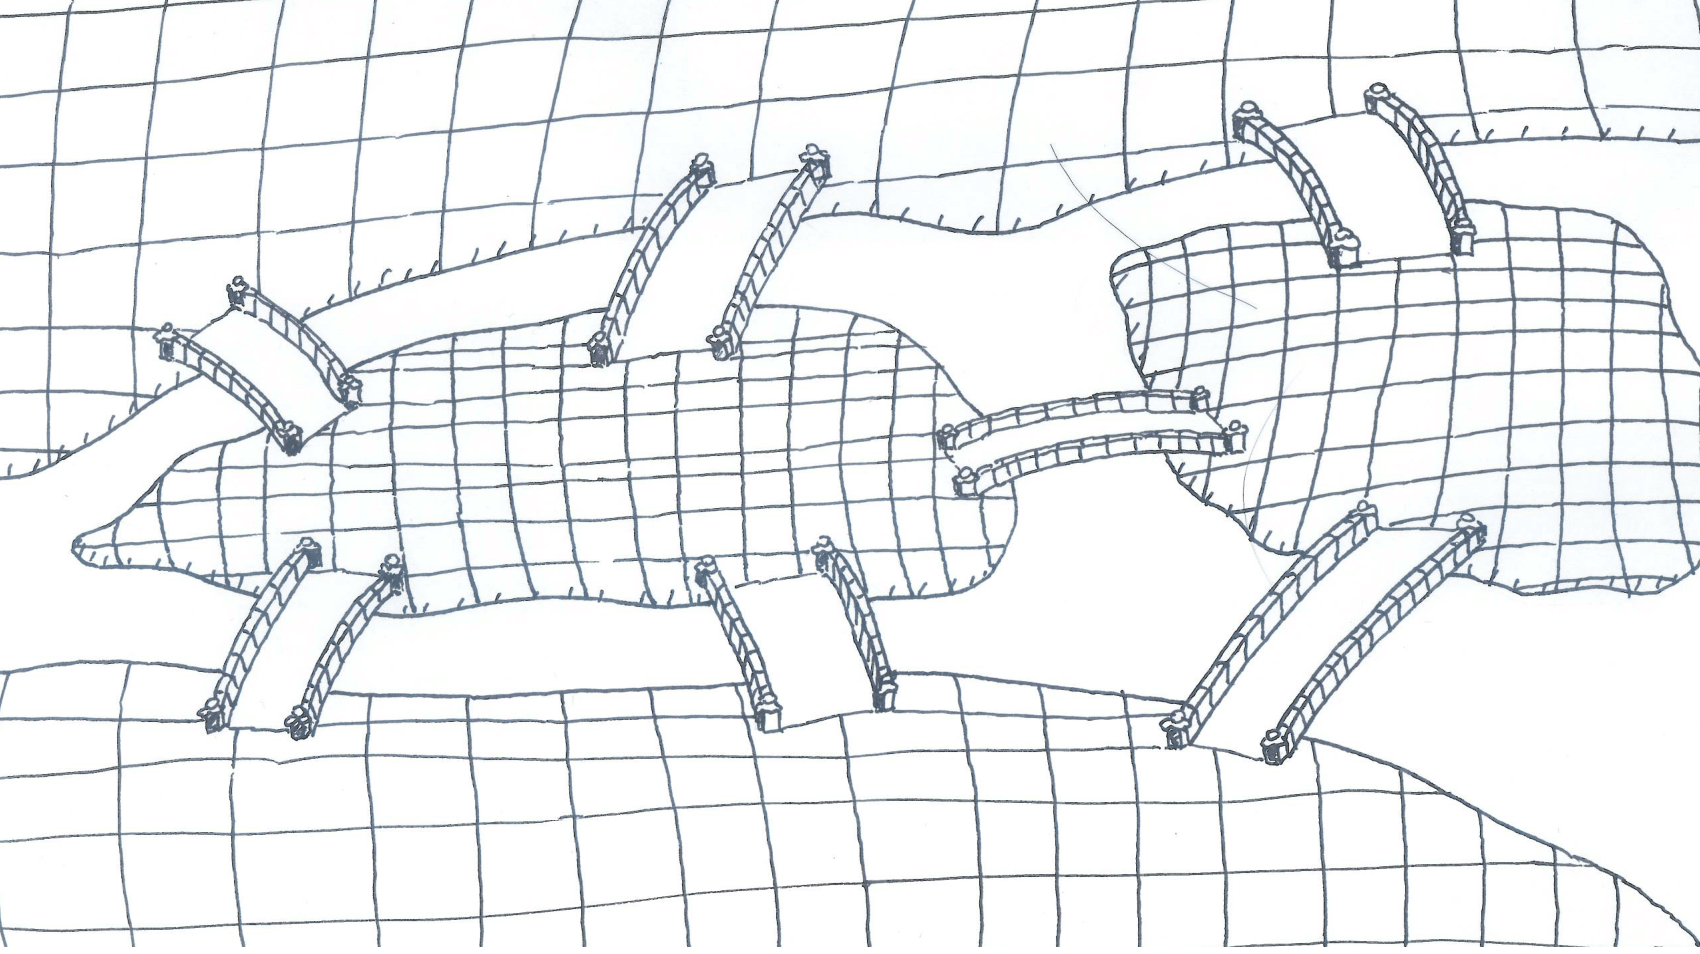
\includegraphics[width=8cm, height=9cm,keepaspectratio]{sections/images/Keningsberg}
\;\ \;\ \;\ \;\ \;\ \;\ \;\ \;\ \;\ \;\
\begin{tikzpicture}
	\tikzstyle{every node}=[circle, draw, fill=red, inner sep=0pt, minimum width=6pt]
    	  
   	\path (0, 0) edge [bend right=45, line width=0.25mm](2, 2)
    	  (0, 0) edge [bend left=45, line width=0.25mm] (2, 2)
    	  (0, 0) edge [bend right=45, line width=0.25mm](2, -2)
    	  (0, 0) edge [bend left=45, line width=0.25mm] (2, -2);	
    	  
	\draw (0, 0) edge [line width=0.25mm] (4, 0)
		  (2, 2) edge [bend left=45, line width=0.25mm] (4, 0)
		  (2, -2) edge [bend right=45, line width=0.25mm] (4, 0);
	
    \draw (0, 0) node {} 
    	  (2, -2) node {} 
    	  (2, 2) node {} 
    	  (4, 0) node {};

\end{tikzpicture}\end{center}

\begin{center}\small Рис. $8$. Кёнигсберг: схематически (слева) и графически (справа)\end{center}

	Эйлер в своей работе не только решил эту задачу, но и сформулировал критерий эйлеровости графа, что позволяет ответить на вопрос для любого графа: можно ли пройти по всем его рёбрам ровно один раз или нет. 
	
	Попробуте обойти следующий граф, а потом посчитайте количество рёбер, которое выходит из каждой вершины. Какое оно?
	
\begin{center}\begin{tikzpicture}
	\tikzstyle{every node}=[circle, draw, fill=blue, inner sep=0pt, minimum width=6pt]
    	  
	\draw (1, 2) -- (4, 7)
		  (1, 2) -- (6, 5);
		  
	\draw (1, 6) -- (4, 7)
		  (1, 6) -- (6, 5);

	\draw (4, 7) -- (4, 1)
		  (4, 7) -- (8, 6);

	\draw (4, 1) -- (6, 5)
		  (4, 1) --(8, 6)
		  (4, 1) -- (7, 2);
		  
	\draw (6, 5) -- (7, 8)
		  (6, 5) -- (8, 9)
		  (6, 5) -- (10, 4);
		  
	\draw (7, 2) -- (11, 6);
	
	\draw (7, 8) -- (8, 9);

	\draw (8, 6) -- (11, 6)
		  (8, 6) -- (8, 9);
		  
	\draw (8, 9) -- (9, 9)
		  (8, 9) -- (11, 6)
		  (8, 9) -- (10, 4);
		  
	\draw (9, 9) -- (11, 6);
	
	\draw (10, 4) -- (11, 6)
		  (10, 4) -- (11, 8);
		  
	\draw (11, 6) -- (11, 8)
		  (11, 6) -- (12, 6)
		  (11, 6) -- (13, 2);
		  
	\draw (12, 6) -- (13, 2);
	
    \draw (1, 2) node {} 
    	  (1, 6) node {} 
    	  (4, 7) node {} 
    	  (4, 1) node {} 
    	  (6, 5) node {} 
    	  (7, 2) node {} 
    	  (7, 8) node {} 
    	  (8, 6) node {} 
    	  (8, 9) node {} 
    	  (9, 9) node {} 
    	  (10, 4) node {} 
    	  (11, 6) node {} 
    	  (11, 8) node {} 
    	  (12, 6) node {} 
    	  (13, 2) node {};

\end{tikzpicture}\end{center}

\begin{center}\small Рис. $9$. Эйлеров граф\end{center}	
	
	Эйлеровы графы имеют в качестве <<собратьев по несчастью>> гамильтоновы графы~---~графы, в которых можно обойти все вершины, побывав в каждой ровно один раз. Однако несмотря на простоту первых из них, вторые не поддаются никакой классификации и до сих пор неизвестно, есть ли оптимальный алгоритм, который мог бы ответить на вопрос: гамильтонов ли наш граф или нет? Говоря об оптимальности, математики подразумевают достаточно формальные понятия. О них мы тоже упомянем немного ниже.
	
	Своим появлением гамильтонов цикл обязан задаче о коммивояжёре, в которой торговец должен был обойти все города, побывав в каждом ровно один раз. С тех пор появилось много задач, для решения которых нужно найти гамильтонов цикл, так что можно считать, что этот путь развития теории графов был вполне успешным.	
	
	Сам Гамильтон сформулировал и решил следующую задачу: можно ли обойти додекаэдр, побывав в каждой вершине единожды. Одно из решений есть на рис. 10.
	
\begin{center}\begin{tikzpicture}
	\tikzstyle{every node}=[circle, draw, fill=red, inner sep=0pt, minimum width=6pt]	
	
	\draw [line width=0.7mm] (126:0.5) -- (198:0.5) -- (270:0.5) -- (342:0.5) -- (342:1.0) -- (18:1.4) -- (18:2.0) -- (90:2.0) -- (162:2.0) -- (234:2.0) -- (306:2.0) -- (306:1.4) -- (270:1.0) -- (234:1.4) -- (198:1.0) -- (162:1.4) -- (126:1.0) -- (90:1.4) -- (54:1.0) -- (54:0.5) -- (126:0.5);

    \draw [dashed]  \foreach \x in {54,126,...,342}
    {
    	
    	(\x:1.0) -- (\x:0.5) -- (\x+72:0.5)
    	(\x-36:1.4) -- (\x:1.0) -- (\x+36:1.4) -- (\x+36:2.0) -- (\x-36:2.0)
    };	
    \draw \foreach \x in {54,126,...,342}
    {
    	(\x:0.5) node {}
    	(\x:1.0) node {}
    };
    \draw \foreach \x in {18,90,...,306}
    {
    	(\x:1.4) node {}
    };
    \draw \foreach \x in {18,90,...,306}
    {
    	(\x:2.0) node {}
    };
\end{tikzpicture}

	\small Рис. 10. Гамильтонов цикл в додекаэдре
\end{center}
	
\begin{paracol}{2}
	\textbf{Теорема о четырёх красках} утверждает, что любую карту можно раскрасить в четыре цвета так, что любая страна раскрашена в один цвет, а соседние страны всегда раскрашены в разные цвета. Фрэнсис Гутри, сформулировавший эту задачу, изначально имел перед собой цель только раскрасить карту Англии. Он заметил, что меньше четырёх красок не хватит для этого. Можете ли вы посмотреть на схематический рисунок Великобритании и объяснить, почему меньше четырёх красок не хватит?
	
	В $1976$ году эту теорему успешно доказали Кеннет Аппел и Вольфганг Хакен, однако то решение, которое они предложили, вызвало сильный резонанс среди коллег. Дело было в том, что математики свели доказательство к проверке около двух тысяч графов на раскраску, но очень трудоёмко~---~проверять все эти случаи вручную, поэтому был написан машинный код, который и должен был справиться с задачей. Такой подход вызвал бурю возмущений среди их коллег...
\switchcolumn
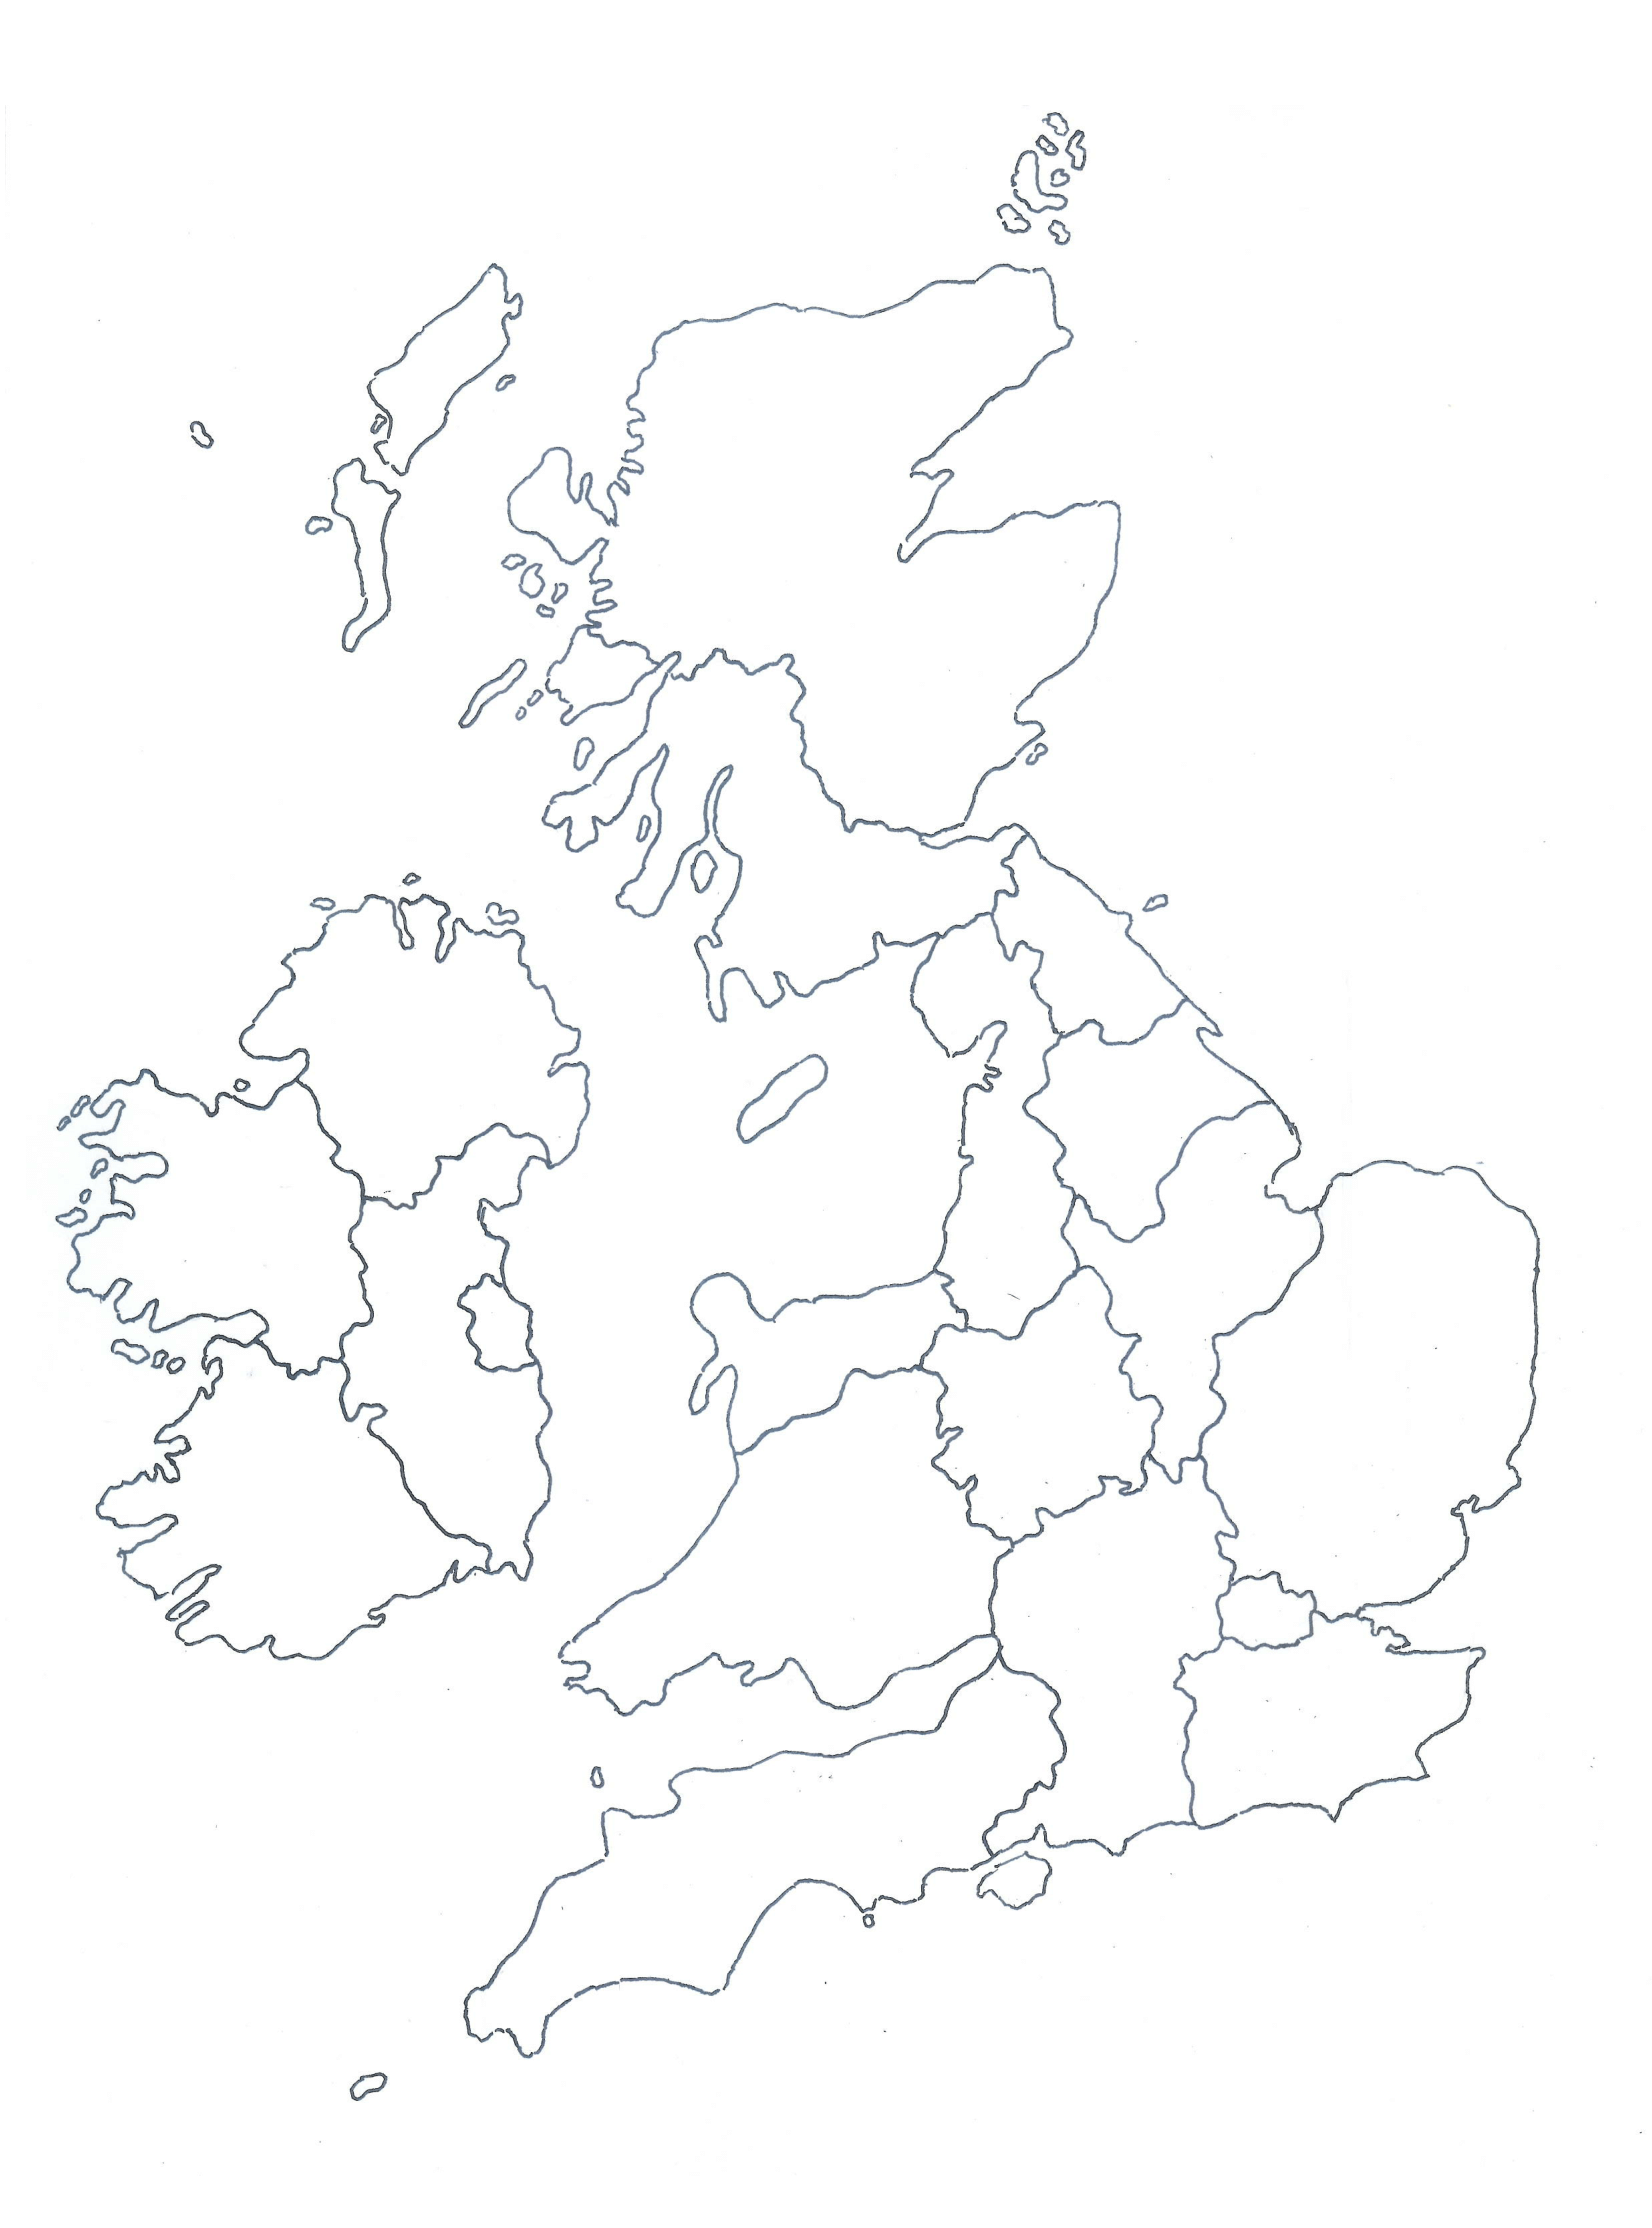
\includegraphics[width=8cm, height=24cm,keepaspectratio]{sections/images/England}
\begin{center}\small Рис. 11. Схематическое изображение частей Великобритании (пропорции не сохранены)\end{center}
\end{paracol}

	Фактически Аппел и Хакен поставили перед научным миром непростой вопрос: можно ли считать доказательство, использующее работу компьютера, строгим, правильным, с формальной точки зрения? 
	
	Долгое время всё сообщество не могло принять такой подход даже по отношению к теореме о четырёх красках, но в $1997$ году Робертсон, Сандерс, Сеймур и Томас предложили более простое доказательство теоремы, которое безвозвратно поместило эту теорему в список <<доказанных>>. К настоящему моменту почти все математики согласились с обоснованным использованием электронных носителей для завершения доказательства сложных теорем.
	
	\textbf{Задача о клике} была сформулирована в $1972$ году Ричардом Карпом. Причиной её появления можно считать дикое развитие теории вычислительных систем, начавшееся в середине $50$-х годов XX века и продолжающееся до сих пор. Условие у этой задачи следующее: предложите оптимальный алгоритм по нахождению максимального полного подграфа произвольного графа. Под полным подграфом подразумевается граф, в котором любые две вершины соединены ровно одни ребром и нет петель, то есть рёбер выходящих и входящих в одну и ту же вершину.
	
	По своей сути задача о клике говорит об оптимальном алгоритме. Ясно, что можно перебрать все возможные подграфы и проверить для каждого, является ли он полным, однако это не будет оптимальным алгоритмом. Критерий оптимальности в этом случае состоит в том, что время, которое мы тратим на работу алгоритма, есть функция, зависящая от длины входных данных. И по этому делению задача о клике относится к $NP$-полным задачам. В этот класс входят те задачи, которые за полиномиальное время не решаются, но любое их решение можно проверить на правильность за полиномиальное время.
	
\begin{center}\begin{tikzpicture}
	\fill [draw=none, fill=green!40] (2, -0.5) -- (3, -1) -- (3, 0) -- (2, -0.5);
	\fill [draw=none, fill=blue!40] (5, -2.5) -- (3, -1) -- (3, 0) -- (5, -1.5);
	\fill [draw=none, fill=green!40] (3, -1) -- (3, 0) -- (7, -0.5);
	\fill [draw=none, fill=red!40] (2, -0.5) -- (3, -1) -- (2.5, -2.5) -- (1.5, -2.5)  -- (0.5, -1.5);
	\fill [draw=none, fill=green!40] (5, -1.5) -- (5, -2.5) -- (8, -2);
	
	\begin{scope}
		\clip (5, -2.5) -- (3, -1) -- (3, 0) -- (5, -1.5);
		\clip (3, -1) -- (3, 0) -- (7, -0.5);
		\fill[color=cyan!80] (3,0) rectangle (5,-2);
	\end{scope}	
	
	\draw (2, -0.5) edge [dashed, line width=0.35mm] (3, -1) 
		  (3, -1)   edge [dashed, line width=0.35mm] (3, 0) 
		  (3, 0)    edge [dashed, line width=0.35mm] (2, -0.5);

	\draw (3, -1)   edge [dashed, line width=0.35mm] (7, -0.5) 
		  (3, 0)    edge [dashed, line width=0.35mm] (7, -0.5);
	
	\draw (3, 0)    edge [dashed, line width=0.35mm] (5, -1.5) 
		  (5, -1.5) edge [dashed, line width=0.35mm] (5, -2.5) 
		  (5, -2.5) edge [dashed, line width=0.35mm] (3, -1)
		  (3, 0)  edge [line width=0.35mm] (5, -2.5) 
		  (3, -1) edge [line width=0.35mm] (5, -1.5);

	
	\draw (2, -0.5)   edge [dashed, line width=0.35mm] (0.5, -1.5) 
		  (0.5, -1.5) edge [dashed, line width=0.35mm] (1.5, -2.5) 
		  (1.5, -2.5) edge [dashed, line width=0.35mm] (2.5, -2.5)
		  (2.5, -2.5) edge [dashed, line width=0.35mm] (3, -1)
		  (2, -0.5)   edge [line width=0.35mm] (1.5, -2.5) 
		  (2, -0.5)   edge [line width=0.35mm] (2.5, -2.5)
		  (0.5, -1.5) edge [line width=0.35mm] (3, -1) 
		  (0.5, -1.5) edge [line width=0.35mm] (2.5, -2.5)
		  (1.5, -2.5) edge [line width=0.35mm] (3, -1);
		  
	\draw (5, -1.5) edge [dashed, line width=0.35mm] (8, -2) 
		  (5, -2.5) edge [dashed, line width=0.35mm] (8, -2);

	\draw (8, -2) edge [line width=0.35mm] (7, -0.5);
		  
	\draw (2, -0.5)   node[circle, draw, fill=white] {1}
		  (3, 0)      node[circle, draw, fill=white] {2}
		  (5, -1.5)   node[circle, draw, fill=white] {3}
		  (3, -1)     node[circle, draw, fill=white] {4}
		  (8, -2)     node[circle, draw, fill=white] {10}
		  (7, -0.5)   node[circle, draw, fill=white] {6}
		  (5, -2.5)   node[circle, draw, fill=white] {7}
		  (0.5, -1.5) node[circle, draw, fill=white] {8}
		  (1.5, -2.5) node[circle, draw, fill=white] {9}
		  (2.5, -2.5) node[circle, draw, fill=white] {5};
\end{tikzpicture}

	\small Рис. 12. Произвольный граф с изображенными кликами
\end{center}

	Это далеко не все задачи, которые встречались по ходу развития теории графов. К ним также можно отнести гипотезу Хадвигера, гипотезу Харари, гипотеза Конвея о трекле.
	
	Подытожим, в этом параграфе мы проследили за процессом становления теории графов, познакомились с неформальным определением графа и обсудили некоторые серьёзные теоремы, с которыми сталкивались математики по мере развития теории графов.
	\section{О неопределяемых понятиях}

\epigraph{\itshape Математика – это больше чем наука, это язык науки.}
{--- Нильс Бор, \textit{создатель квантовой теории атома}}

	Чтение этого параграфа будет полезно тем, кто не работал еще с теорией множеств и теорией отображений. Конечно, после чтения этих
	пары страниц читатель не станет гением в этой области, но это поможет ему с меньшим напряжением осилить следующую главу.

\mysubsection{Обозначения}

	В первую очередь, я решил указать списком все обозначения, которые мы дальше будем использовать в надежде на то, 
	что читатель, наткнувшийся на непонятный для него знак в тексте, сможет обратится к этому списку и обновить свои знания.
	
\begin{itemize}
\item $\Rightarrow$~---~следствие, импликация; $A \Rightarrow B$ означает, что если верно $A$, то верно и $B$,
\item $\Leftrightarrow$~---~равносильность, эвивалентсность; $A \Leftrightarrow B$ означает, что $A$ верно тогда и только тогда, когда верно $B$, 
\item $\wedge$~---~конъюнкция, знак <<и>>; $A \wedge B$ истинно тогда и только тогда, когда и $A$, и $B$ истинны,
\item $\vee$~---~дизъюнкция, знак <<или>>; $A \vee B$ истинно, когда $A$ истинно или $B$ истинно,
\item $\neg$~---~отрицание; $\neg A$ истинно, если $A$ ложно,
\item $\forall$~---~квантор всеобщности, <<для каждого>>; $\forall \!\ a, P(a)$ означает, что для всякого $a$ верно $P(a)$,
\item $\exists$~---~квантор существования, <<существует>>; $\exists \!\ a, P(a)$ означает, что существует такое $a$, что $P(a)$ верно,
\item $\exists!$~---~<<существует единственый>>; $\exists! \!\ a, P(a)$ означает, что существует единственное такое $a$, что $P(a)$ верно,
\item $\colon$~---~такое, что; $a: P(a)$ означает, что мы рассматриваем только такие $a$, что $P(a)$ верно,
\item $\colon=$~---~по определению равно; $a \colon = b$ означает, что по определению $a$ равно $b$,
\item $\mapsto$~---~выполняется; $\forall \!\ a \mapsto P(a)$ означает, что для любого $a$ верно $P(a)$,
\item $\displaystyle\sum$~---~сумма; $\displaystyle\sum_{a \in A} P(a)$ равно сумме значений $P(a)$,
\item $\displaystyle\prod$~---~произведение; $\displaystyle\prod_{a \in A} P(a)$ равно произведению значений $P(a)$.
\end{itemize}
	
\mysubsection{Множества}

	Вспомним уроки геометрии в школе, где, возможно, не всем из нас, но многим приходилось учить аксиомы планиметрии 
	или просто сталкивался с ними. Кроме этих аксиом, также были и неопределяемые понятия: например, точка, плоскость. 
	И это не исчерпывает список того, что закладывается в фундамент математики: нам также, не объясняя, говорили о принципе 
	наложения фигур друг на друга.
	
	Есть отдельные области в математики, которые занимаются обсуждением того, что лежит в самых низах теорий. К ним можно отнести 
	и теорию множеств, и теория моделей, и теорию доказательств. За всеми этими словами стоят гигантские тексты, в которых изложено 
	неизмеримое множество утверждений. Мы не будем вдаваться во всё это, а остановимся на том материале, который нам позволит 
	грамотно воспринимать всю оставшуюся книгу.
	
	Суть множества~---~набор элементов, не имеющий никакой структуры. Сами элементы могут иметь произвольную природу. 
	Будем говорить, что \emph{элемент $a$ принадлежит множеству $A$}, если $a$ присутствует в наборе элементов этого множества, 
	и писать $a \in A$. Множество однозначно задается своими элементами, то есть $A = B$ тогда и только тогда, 
	когда любой элемент $A$ принадлежит множеству $B$, и наоборот.
	
	Заметим, что в определении множества мы использовали двойное вложение, то есть $A \subseteq B$ и $B \subseteq A$. 
	В общем случае множество $A$, вложенное в множество $B$, называется его \emph{подмножеством}.
	
	Отдельно уточним то, что каждый элемент может представлять из себя тоже отдельное множество. В этом смысле множества 
	могут походить на функциональный язык LISP, после работы с которым в кошмарах программиста еще долго будут сниться круглые скобочки.
	
	Важно помнить, что обозначения, которыми пользуются, чтобы показать вложимость множеств
	или принадлежность элемента множеству, от раза к разу могут означать разное. Однако, исходя
	из банальных правил логики, можно вывести смысл некоторых обозначений.
	
	Например, под $A \subseteq B$ мы будем подразумевать, что множество $A$ подмножество $B$ 
	и при этом оно может совпадать с $B$. В противном случае, чтобы показать, что подмножество
	является \emph{собственным} или простыми словами: не может совпадать со всем множеством, ---
	пишут так $A \subset B$. Иногда можно встретить еще такое обозначение, имеющее такой же смысл,
	что и предыдущее: $A \subsetneq B$.	
	
	Помимо этого, используется также обозначение $a \notin A$, если $a$ нет в множестве $A$ 
	(хочется отметить, что иногда это обозначение используют в диком смысле, подразумевая, например,
	что $a$ тоже множество или объект <<другой природы>> нежеле элементы множества $A$).
	
\begin{testquestion}
	Пусть $A = \{ 1, 2, 3, 4\}$, $B = \{3, 4, 5, 6\}$, $C = 3$. 
	
	Верно ли, что $C \in A$ и $C \subseteq B$? А то, что $B \notin A$?
\end{testquestion}	

	Нам будут встречаться \emph{числовые множества}:
	
\begin{itemize}
	\item натуральные числа ($\BN$)~---~$1, 2, 3, 4, 5, 6, 7, 8, 9, \dots$
	\item целые числа ($\BZ$)~---~$\dots, -4, -3, -2, -1, 0, 1, 2, 3, 4, 5, 6, \dots$
	\item простые числа ($\BP$)~---~$2, 3, 5, 7, 11, 13, 17, 19\dots$
	\item рациональные числа ($\BQ$)~---~$\dots,\frac{1}{2}, 2, 3, -\frac{3}{17}, -5, \frac{4}{53}, 0.(3), \dots$
	\item действительные числа ($\BR$)~---~$\dots,e, -\frac{1}{2}, 16, -\sqrt{3}3, -\frac{17}{3}, -5, \frac{4}{53}, 0.(3), \pi, \dots$
	\item комплексные числа ($\BC$)~---~$\dots, ie, 1 + i, 16i, -\sqrt{-3}3, -\frac{5}{24}, -7, \frac{97}{53 + i}, \frac{2+i}{3+i}, \pi + i, \dots$
\end{itemize}
	
	Иногда к числовым множествам приписывают индексы и степени, например, под $\BN_0$ подразумевается множество натуральных чисел и ноль. Или если мы пишем $\BR_{\geqslant 0}$, то это множество неотрицательных действительных чисел.	
	
	А некоторые множества мы будет сами перечислять, то есть, например, множество покупок в продуктовом может выглядеть следующим образом
	$$\lbrace \text{мясо}, \:\ \text{апельсины}, \:\ \text{гречка}, \:\ \text{молоко}, 
	\:\ \text{овощи}, \:\ \text{рыба}, \:\ \text{хлеб}, \:\ \text{квас}, \dots \rbrace.$$
	
	А множество оценок, которые ставит преподаватель в течение года, будет выглядеть так
	$$\lbrace 5, 4, 3, 2, 1\rbrace.$$
	
	Заметим, что элементы множества могут быть, например, \emph{кортежами} --- упорядоченными наборами чисел (в отличие от множеств их обычно заключают в круглые скобочки)
	$$\{ (1, 2, 3), (2, 4, 45), (13, -7, 15), (34, -10, 1) \}.$$	
	
	\emph{Пустое множество} не содержит ни одного элемента и обозначается $\varnothing$.
	
\begin{testquestion}
	Сколько элементов в множестве $\lbrace \lbrace 1, 3\rbrace, 4, \lbrace 2, 4, 5\rbraceб \varnothing \rbrace$?
\end{testquestion}	

	Кроме явных представлений множеств, их также можно определить посредством введения условий, 
	которое обычно пишут в окружении фигурных скобок. Например, множество элементов, кратных числу $p$ обозначается так
	$$p\BZ = \lbrace a \colon a=pk, k \in \BZ\rbrace.$$

	Или обычным заданием множеств будет приписывание эпитетов или дополнений к самому слову <<множество>>:
\begin{center}
	множество подмножеств, минимальное множество.
\end{center} 

\begin{testquestion}
	Как называется это множество: $\lbrace a \colon a^2 + 1 = 0, a \in \BR\rbrace$?
\end{testquestion}	
	
	
	Заметим, что далее мы будем подразумевать, что имеем дело с обычными, а не \emph{мультимножествами}, 
	в которых допускается повторение элементов. К тому же нельзя забывать о том, что главное отличие множества от 
	кортежа в том, что оно не упорядочено, то есть 
	$$\lbrace 5, 4, 3, 2, 1\rbrace = \lbrace 3, 2, 4, 5, 1\rbrace = \lbrace 1, 2, 3, 4, 5\rbrace = \lbrace 4, 5, 3, 1, 2\rbrace.$$
	
\mysubsection{Операции на множествах}	
	
	Множества подобны существительным в языке. Именно так же, как и последние нуждаются в глаголах, 
	множества нуждаются в операциях, которые и определяли бы всю дальнейшую работу с ними.
	
	\emph{Объединением множеств $A$ и $B$} называется множество, состоящее из элементов множества $A$ и множества $B$, 
	и обозначается $A \cup B$. Другими словами,
	$$a \in A \cup B \Leftrightarrow a \in A \vee a \in B.$$
	
	\emph{Пересечением множеств $A$ и $B$} называется множество, состоящее из элементов, которые встречаются как в $A$, 
	так и в $B$, и обозначается $A \cap B$. Иначе говоря,
	$$a \in A \cap B \Leftrightarrow a \in A \wedge a \in B.$$
	
	\emph{Разностью множеств $A$ и $B$} называется множество, состоящее из элементов, которые встречаются в $A$, 
	но не встречаются в $B$, и обозначается $A \backslash B$:
	$$a \in A \backslash B \Leftrightarrow a \in A \wedge a \notin B.$$
	
	Также отдельно выделяют \emph{симметрическую разность множеств $A$ и $B$}, подразумевая под ней 
	$(A \backslash B) \cup (B \backslash A)$ и обозначая $A \bigtriangleup B$. И еще, чтобы сократить
	немного запись, объединение непересекающихся множеств обозначают $A \sqcup B$ и называют
	\emph{дизъюнктным объединением}.
	
\begin{testquestion}
	Что это за множество $(\BZ \bigtriangleup \BN) \cup \BN$?
\end{testquestion}

\begin{testquestion}
	Пусть $A$ и $B$ содержат по $5$ элементов. Что можно тогда сказать про мощность $A \bigtriangleup B$?
\end{testquestion}

	Еще есть \emph{декартово произведение $A \times B$}~---~это множество упорядоченных пар $(a, b)$ таких, 
	что $a \in A$, а $b \in B$. Часто используют обозначение $A^n$ для множества, полученного декартовым произведением $A$ множеств $n$ раз.
	
\mysubsection{Отображения}
	
	По сути \emph{отображение $f$} есть ни что иное, как правило, по которому мы каждому элементу множества $A$ ставим в 
	соответствие единственный элемент множества $B$. В таком случае принято обозначение $f: A \to B$.
	
	Среди всевозможных отображений $f: A \to B$ выделяют следующие три их вида:

\begin{enumerate}
	\item \emph{инъекция}: $\forall \!\ a_1, a_2 \in A \colon a_1 \neq a_2 \mapsto f(a_1) \neq f(a_2)$,
	\item \emph{сюръекция}: $\forall \!\ b \in B \exists \!\ a \in A \colon f(a) = b$,
	\item \emph{биекция}: $\forall \!\ b \in B \exists! \!\ a \in A \colon f(a) = b$.
\end{enumerate}

\begin{testquestion}
	Каким будет отображение $f: \BN \to \BN, f(n) = 2n$?
\end{testquestion}

\begin{testquestion}
	Каким будет отображение $f: \BR \to \BR, f(x) = x \cdot \sin(x)$?
\end{testquestion}

	В речи и письме часто употребляют понятия: \emph{образ} $a$, подразумевая $f(a)$; \emph{прообраз} $b$, 
	подразумевая $a \in A \colon f(a) = b$; \emph{образ отображения}~---~подмножество $B$, состоящее из всех образов элементов из $A$.
	
\begin{testquestion}
	Какие из нижеперечисленных отображений из множества $A = \{ 1, 2, 3, 4\}$ на множество $B = \{ 10, 20, 30, 40\}$ являются биекциями?
	$$f_1\colon x \mapsto 10(5-x), f_2\colon x \mapsto 10x, f_3\colon x \mapsto 10 (x-2)^2.$$
\end{testquestion}
	\section{О степенях вершин и числе рёбер}
	
\mysubsection{Простой граф, псевдограф, мультиграф}	
	
	В первую очередь, дадим теперь уже совершенно строгое определение графа.

\begin{definition}
	\emph{Граф}~---~два упорядоченных множества: конечного множество вершин $V$ (от англ. vertex), 
	конечного множество рёбер или дуг $E$ (от англ. edge) и отображение инцидентности $I: E \to V^2$. 
	Обозначается обычно так $G = \langle V, E, I\rangle$ или $G(V, E)$.
\end{definition}

	Для тех, кто в <<танке>>, скажу немного про отображение инцидентности. Если сопоставление само по 
	себе~---~это правило, по которому каждому элементу множества $A$ ставится в соответствие элемент множества $B$, 
	то в случае инцидентного отображения каждому ребру сопоставлено какая-то пара вершин, которые оно соединяет.

\begin{paracol}{2}
\begin{example}
	Справа вы можете увидеть представителя выпуклых многоугольников, а именно~---~треугольника. Но нас будет 
	интересовать не геометрическая, а теоретико-графовая конструкция. В терминах графов его можно обозначить так:
	$$G(\lbrace a, b, c\rbrace, \lbrace \lbrace a, b\rbrace, \lbrace b, c\rbrace, \lbrace c, a\rbrace \rbrace).$$
\end{example}

\switchcolumn

\begin{center}\begin{tikzpicture}
	\draw (-0.2, -1.2) node [left] {a}
		  (0.8, 2.2) node [above] {b}
		  (4.2, -0.2) node [right] {c};	

	\tikzstyle{every node}=[circle, draw, fill=red, inner sep=0pt, minimum width=6pt]	
	
	\draw (0, -1) node {} --
		  (1, 2) node {} --
		  (4, 0) node {} -- (0, -1);	
\end{tikzpicture}

	\small Рис. \images. Треугольник
\end{center}
\end{paracol}
\refstepcounter{images}

	Заметим, что нигде не было сказано, что точки должны располагаться на плоскости. На самом деле граф 
	можно расположить и в пространстве. Например, каркасы любых многогранников представляют из себя графы.

	Уточним определение графа: если под множеством $V^2$ подразумевается множество упорядоченных пар вершин, то граф 
	называется \emph{ориентированным}. В противном случае он будет \emph{неориентированным}. Впоследствии там, где будут встречаться 
	ориентированные графы, мы их будем обозначать буквой $D$, а в остальных случаях будем пользоваться буквой $G$.

	Для того чтобы было понятно, в каком случае у нас ребро ориентировано, а в каком~---~нет, введём обозначение: 
	$\left\lbrace a, b \right\rbrace$~---~это неориентированное ребро, а $(a, b)$ или $(b, a)$~---~ориентированное.
	
\begin{definition}
	Рёбра называются \emph{кратными}, если они соединяют одни и те же вершины (и в том же порядке для ориентированных рёбер). 
	Также говорят, что вместе кратные рёбра образуют \emph{мультиребро}. Граф, в котором разрешены мультирёбра, называется \emph{мультиграфом}.
\end{definition}

	Еще раз хочу остановить внимание читателя на том, что кратными также могут быть и ориентированные рёбра, но в этом случае 
	важно не только то, что они соединяют одни и те же вершины, но и их порядок. Кроме того, мы ничего не говорим 
	про кратность ребра, то есть в мультиребро может входить как два, так и три, четыре и большее количество ребер.

\begin{definition}
	Ребро называется \emph{петлей} (loop), если оно соединяет вершину саму с собой. 
	Граф, в котором разрешены петли называется \emph{псевдографом}.
\end{definition}

	Эти понятия можно комбинировать, получая по истине удивительные словообразования: 
	псевдомультиграф, мультиорграф, псевдоорграф, псевдомультиорграф.

	Для того чтобы закрепить понимания читателем отображение инцидентности, рассмотрим следующий пример, после которого 
	мы наконец перейдем к простым графам, в которых нам уже не понадобится это отображение (хочу отметить, что в более 
	общей теории нельзя опускать это понятие, но мы пока что изучаем самые азы, поэтому можем пренебречь этим).

\begin{example}
	Отображение инцидентности $I$ можно задать в виде таблице, в которой в первой строке будут выписаны ребра, 
	а во второй~---~соответствующие им пары вершин:

\begin{center}
 \begin{tabular}{||c|c|c|c|c|c|c|c|c||} 
 \hline
 $E$ & $a$ & $b$ & $c$ & $d$ & $e$ & $f$ & $g$ & $h$ \\
 \hline
 $V \times V$ & $\lbrace1, 2\rbrace$ & $\lbrace1, 2\rbrace$ & $\lbrace2, 3\rbrace$ & $\lbrace2, 3\rbrace$ & 
 $\lbrace3, 4\rbrace$ & $\lbrace4, 5\rbrace$ & $\lbrace5, 5\rbrace$ & $\lbrace5, 1\rbrace$ \\ 
 \hline
\end{tabular}\end{center}

	Ей соответствует граф $G$, изображенный на рис. 17.

\begin{center}\begin{tikzpicture}
	\Loop (-2, 2) [dir=WE];	
	
	\node at (0, 0)[below left]{$1$};  
	\node at (4, 0)[below right]{$2$};  
	\node at (4, 4)[above right]{$3$};  
	\node at (0, 4)[above left]{$4$};  
	\node at (-2, 1.8)[below]{$5$};
	
	\node at (2, 0.3){$a$};  
	\node at (2, -0.7){$b$};  
	\node at (3.3, 2){$c$};  
	\node at (4.7, 2){$d$};  
	\node at (2, 4.3){$e$};
	\node at (-1.2, 3.2){$f$};  
	\node at (-4.5, 2){$g$};  
	\node at (-0.8, 1.2){$h$};
	
	\node at (6, 0) {};  
	
	\tikzstyle{every node}=[circle, draw, fill=red, inner sep=0pt, minimum width=6pt]
	[line width=2pt]
	\draw (0, 0) edge [line width=1pt] (4, 0);
	\draw (0, 0) edge [bend right = 25, line width=1pt] (4, 0);
	\draw (4, 0) edge [bend right = 25, line width=1pt] (4, 4);
	\draw (4, 0) edge [bend left = 25, line width=1pt] (4, 4);
	\draw (4, 4) edge [line width=1pt] (0, 4);
	\draw (0, 4) edge [line width=1pt] (-2, 2);
	\draw (-2, 2) edge [line width=1pt] (0, 0);
	
	\node at (0, 0){};  
	\node at (4, 0){};  
	\node at (4, 4){};  
	\node at (0, 4){};  
	\node at (-2, 2){};
\end{tikzpicture}\end{center}
\begin{center}
	\small Рис. \images. Пример псевдомультиграфа 
\end{center}

\end{example}

\begin{paracol}{2}
\begin{definition}
	Неориентированный граф называется \emph{простым}, если он не содержит петель и кратных ребер.
\end{definition}

	Везде дальше мы будем подразумевать по умолчанию, что работаем только с простыми графами. Из-за этого 
	мы фактически не будем использовать отображение инцидентности, подразумевая, что $E~\subset~V~\times~V$.
	
	Справа, на рис. 18, изображен граф Петерсона, который в свое время стал одним из самых известных примером непланарного графа.

\switchcolumn

\begin{center}\begin{tikzpicture}
	\tikzstyle{every node}=[circle, draw, fill=red, inner sep=0pt, minimum width=6pt]
	\foreach \x in {18,90,...,306}
    {
    	\draw
    	(\x:1.5) node {} -- (\x+144:1.5)
    	(\x:1.5) node {} -- (\x+216:1.5);
    };
    \foreach \x in {18,90,...,306}
    {
    	\draw
    	(\x:2.5) node {} -- (\x:1.5)
    	(\x:2.5) node {} -- (\x+72:2.5);
    };
    \draw \foreach \x in {18,90,...,306}
    {
    	(\x:1.5) node {}
    };
    \draw (18: 2.5) node {};
\end{tikzpicture}\end{center}
\begin{center}
	\small Рис. \images. Пример простого графа 
	
	(граф Петерсена)
\end{center}
\end{paracol}
\refstepcounter{images}

\begin{definition}
	\emph{Полный граф}~---~простой граф, в котором любые две вершины соединены ребром. Обозначение: $K_n$.
\end{definition}

\begin{example}
	Сколько ребер в полном графе $K_n$? Сколько различных графов мы можем получить из него, стирая некоторые ребра?
	
	К ответу на первый вопрос можно прийти несколькими способами. Например, можно заметить, что между парами вершин и 
	ребрами существует взаимно однозначное соответствие, поэтому количество ребер равно $C_n^2 = \frac{n(n-1)}{2}$. 
	Иначе можно заметить, что из каждой вершины выходит ровно $n - 1$ ребро, а всего вершин у нас~---~$n$. Следовательно, 
	$n(n-1)$~---~это удвоенное количество ребер, так как каждое ребро мы посчитали дважды.
	
	Дальше, чтобы понять, сколько мы можем получить различных графов, стирая ребра, заметим, что ребро может быть либо стерто, либо нет. 
	Таким образом, у каждого ребра два возможных состояния. Поэтому количество искомых графов равно $2^{|E|}$, где $|E|$~---~обозначение 
	для количества ребер в графе. 
\end{example}

\begin{example}[Бабичева Т.С., Бабичев С.Л., Жогов А. А., Яковлев И.В. <<Пособие по олимпиадной математике. Уровень А1>>]
	В Шире между $10$ домами проложено $20$ аккуратных брусчатых дорог, каждая из которых связывает какие-то два дома. 
	Экономящие свое время аккуратные хоббиты хотят проложить еще несколько дорог так, чтобы из каждого дома можно было 
	добраться до любого другого, причем лишних дорог строить не трубется (два дома должна соединять лишь одна дорога). 
	Сколько дорог необходимо еще построить?
	
	\emph{Решение.} После стройки граф дорог будет полным, следовательно, в нем будет 
	$$\frac{10 \cdot (10-1)}{2} = 45 \;\ \text{дорог}.$$
	Так как $20$ дорог уже есть, то осталось проложить еще $25$.
\end{example}

\begin{example}[Бабичева Т.С., Бабичев С.Л., Жогов А. А., Яковлев И.В. <<Пособие по олимпиадной математике. Уровень А1>>]
	Среди $49$ школьников каждый знаком не менее чем с $25$ другими. Докажите, что можно их разбить на группы из $2$ или 
	$3$ человек так, чтобы каждый был знаком со всеми в своей группе.
	
	\emph{Решение.} Рассмотрим максимальное разбиение школьников на такие группы. Допустим, что у кого-то еще нет пары или тройки. 
	Назовем его потерявшимся. Так как среди оставшихся школьников меньше $50$ человек, групп среди них будет не больше $24$~---~а 
	значит, есть группа, в которой у потерявшегося будет двое знакомых.
	
	Если эта группа будет состоять из двух людей, то мы добавляем к ним потерявшегося, иначе мы делим группу вместе с потерявшимся 
	на две пары. В любом случае мы смогли указать большее разбиение. Противоречие. Это означает, что максимальное такое 
	разбиение будет покрывать всех школьников.
\end{example}

\mysubsection{Лемма о рукопожатиях}

\begin{definition}
	Пусть $e = \left\lbrace x, y \right\rbrace \in E$. Тогда говорят, что вершины $x$ и $y$ \emph{инцидентны} ребру $e$, 
	а ребро $e$ \emph{инцидентно} вершинам $x$ и $y$. Часто также говорят, что $x$, $y$~---~\emph{концевые вершины} ребра $e$. 
	Два ребра называются \emph{смежными}, если они имеют общую вершину. Две вершины называются \emph{смежными}, 
	если они инцидентны одному и тому же ребру.
\end{definition}


\begin{definition}
	Количество ребер, выходящих из данной вершины, называется \emph{степенью} или \emph{валентностью} этой вершины. 
	Подразумевается, что петля дает двойной вклад. Вершина графа, имеющая нечетную степень называется \emph{нечетной}, 
	а имеющая четную степень~---~\emph{четной}. Далее степень вершины $a$ будем обозначать через $deg(a)$.
\end{definition}

\begin{statement}
	В любом граве с $n \geqslant 2$ вершинами есть две вершины с одинаковой степенью.
	
\begin{proof}
	От противного. На степень произвольной вершины $a$ есть следующее ограничение
	$$0 \geqslant deg (a) \geqslant n-1.$$
	Если нет двух вершин одинаковой степени, то для любого $k \in [0, n-1], k \in \BN$ найдется вершина,
	у которой степень будет равна $k$. Следовательно, есть вершина нулевой степени, то есть ни с кем не соединенная,
	и вершина со степепенью $n-1$, то есть соединенная со всеми остальныим. Противоречие.
\end{proof}
\end{statement}

	При доказательстве этого утверждения мы пользовались методом Дирихле (самым простым из его видов). Если читатель не знаком с ним,
	то советую уделить время на него, так как он часто применяется в олимпиадных задачах.

	В примере выше мы уже суммировали степени вершин полного графа. Оказывается, что это не безуспешное занятие и в общем случае.

\begin{lemma}[о рукопожатиях]
	Сумма степеней вершин произвольного графа равна удвоенному количеству его ребер.
	
	\emph{Доказательство.} Вообщем-то частично мы уже доказали это утверждение выше. Для полного доказательства заметим, что если 
	мы просуммируем степени всех вершин, то каждое ребро мы учтем дважды, так как у каждого ребра ровно два конца. 
	Таким образом, мы и приходим к следующей формуле $$\sum_{a \in V} deg(a) = 2|E|.$$
\end{lemma}

\begin{consequence}
	Количество нечетных вершин любого графа четно.
\end{consequence}

	Последнее утверждение имеет название <<Лемма о рукопожатиях>>, так как если взять произвольную группу людей, тогда 
	среди них будет всегда четное количество людей, которые в течение дня жали руку нечетному количеству людей из этой же группы. 
	Или, например, за всю историю человечества количество людей, которые жали руку нечетное число раз, четно.

	Несмотря на вполне тривиальную формулировку и доказательство, эта лемма представляет из себя применение одного из сильных методов 
	олимпиадной математики~---~ двойного подсчета (double counting). Смысл этого метода состоит в том, что произвольное множество $M$ 
	можно разбить на непересекающиеся подмножества неединственным образом. Например, допустим, что у нас есть два разбиения 
	$$M = \bigcup_i A_i, \forall \!\ k \neq m \colon \!\ A_k \cap A_m = \varnothing; 
	M = \bigcup_j B_j,  \forall \!\ k \neq m \colon \!\ B_k \cap B_m = \varnothing.$$

	Тогда можно два раза подсчитать, сколько элементов в $M$
	$$\sum_i |A_i| = |M| = \sum_j |B_j|.$$	
	
	В это равенство и заложена суть метода двойного подсчета.
	
	Добавим, что если читатель~---~школьник, который хочет завоевывать дипломы на олимпиадах разного уровня, 
	то ему стоит обратить внимание на метод двойного подсчета, так как он часто встречается в олимпиадах.
	
\begin{example}
	На экскурсию пришло 19 школьников. Могло ли так получится, что каждая девочка знакома ровно с пятью школьниками, 
	а каждый мальчик~---~ровно с тремя школьниками?\\
	
	\emph{Решение.} Заметим, что если школьников обозначить вершинами, а знакомства~---~ребрами, то все 
	вершины окажутся нечетными, но их нечетное число. Противоречие. Следовательно, так не могло быть.
\end{example}

	Целый пласт простых олимпиадных задач решается с помощью применения леммы о рукопожатиях, хотя более экзотическое 
	ее применение можно найти только в совокупности с другими более сильными теоремами. 

\mysubsection{Степенные последовательности}

\begin{definition}
	Назовем последовательность $(d_1, d_2, \dots, d_n)$ \emph{правильной}, если 
	$$n-1 \geqslant d_1 \geqslant d_2 \geqslant \dots \geqslant d_n \;\ \text{и} \;\ \sum_{i=0}^n d_i - \!\ \text{четное число}.$$  
\end{definition}

\begin{definition}
	\emph{Степенная последовательность}~---~это последовательность степеней вершин псевдомультиграфа $G$, записанная в порядке невозрастания. 
	\emph{Графическая последовательность}~---~это правильная последовательность, соответствующая степеням какого-то простому графу.
\end{definition}

	На самом деле тут мы немного схитрили, потому что очевидным образом из леммы о рукопожатиях следует второе условие 
	правильности последовательности, а первое условие~---~из того, что все исходящие ребра соединяют вершину с какой-то еще, 
	то есть их меньше, чем $C_{n-1}^1 = n-1$. 
	
	Степенные и графические последовательности начали изучать в связи с поиском универсальной величины, по которой мы смогли 
	бы отличать графы друг от друга. Но, к сожалению, несмотря на критерий, который мы обсудим ниже, этот путь не привел ни к 
	каким грандиозным результатам.	
	
\begin{statement}[критерий степенной последовательности]
	Последовательность неотрицательных невозрастающих целых чисел $(a_1, a_2, \dots, a_n)$ будет степенной тогда и только тогда, 
	когда сумма чисел в ней четна.
	
\begin{proof}
	Необходимость четности следует из леммы о рукопожатиях. Чтобы показать, что этого условия достаточно, построим такой граф.
	
	Во-первых, возьмем $n$ изолированных вершин и пронумеруем их. Во-вторых, проведем $\lfloor \frac{a_i}{2} \rfloor$ петель у $i$-й вершины, 
	и вычтем из всех $a_i$-х удвоенное число соответствующих петель. Пусть после вычитания получились числа $(b_1, b_2, \dots, b_n)$; 
	каждое из них будет равно либо нулю, либо единице. Однако так как мы вычитали четные числа, то их сумма осталась четна. 
	Следовательно, можно все вершины разбить на пары и соединить ребром в каждой паре. В итоге мы получили граф, 
	у которого степенная последовательность совпадает с исходной.
\end{proof}\end{statement}

	Таким образом, мы можем легко отделить из всех неотрицательных невозрастающих последовательностей те, 
	которые будут степенными. Однако в случае с графическими последовательностями так легко мы уже не отделаемся.

\begin{theorem}[Эрдеша-Галлаи]
	Правильная последовательность $(d_1, d_2, \dots, d_n)$ является графической тогда и только тогда, когда 
	$$\forall \!\ k \in \BN: 1 \leqslant k \leqslant n-1 \mapsto \sum_{i=1}^k d_i \leqslant k(k-1) + \sum_{i=k+1}^n min \lbrace k, d_i \rbrace. $$
\end{theorem}

	Доказательство этой теоремы мы здесь приводить не будем, потому что материал, который нужен для этого, нельзя разместить 
	в одну-две страницы, поэтому если бы мы поступили иначе, то его пришлось бы нещадно сжимать, что привело бы к потере качества.

	Хочется добавить, что есть даже конструктивный подход, а именно~---~алгоритм Гавела-Хакими, который позволяет по 
	произвольной графической последовательности построить граф, который будет иметь такую степенную последовательность.

	К сожалению, несмотря на такие сильные утверждения, как теорема Эрдеша-Галлаи, графическая последовательность не стала 
	ключом к подсчету графов, потому что у разных графов она может совпадать, как в следующем примере.
	
\begin{example}
	Нарисовать три различных графа с графической последовательностью $(3, 2, 2, 1, 1, 1)$.
	
\begin{center}\begin{tikzpicture}
	\tikzstyle{every node}=[circle, draw, fill=red, inner sep=0pt, minimum width=6pt]	
	
	\draw (0, 0) node {} -- (1, 1) node {} -- (2, 1) node {};
	\draw (0, 0) node {} -- (1, 0) node {};
	\draw (0, 0) node {} -- (1, -1) node {} -- (2, -1) node {};	
\end{tikzpicture}
\;\ \;\ \;\ \;\ \;\ \;\ \;\ \;\ \;\ \;\ 
\begin{tikzpicture}
	\tikzstyle{every node}=[circle, draw, fill=red, inner sep=0pt, minimum width=6pt]	
	
	\draw (0, 0) node {} -- (1, 1) node {} -- (-1, 1) node {} -- (0, 0) node {} -- (0, -1) node {};
	\draw (1, -1) node {} -- (2, 0) node {};	
\end{tikzpicture}
\;\ \;\ \;\ \;\ \;\ \;\ \;\ \;\ \;\ \;\ 
\begin{tikzpicture}
	\tikzstyle{every node}=[circle, draw, fill=red, inner sep=0pt, minimum width=6pt]	
	
	\draw (0, 0) node {} -- (1, 0) node {} -- (2, 0) node {} -- (3, 0) node {};
	\draw (0, 0) node {} -- (1, 1) node {};
	\draw (0, 0) node {} -- (1, -1) node {};	
\end{tikzpicture}
\newline
\newline
	\small Рис. \images. Три различных графа с одинаковой степенной последовательностью
\end{center}
\end{example}

Кроме теоремы Эрдеша-Галлаи, есть еще один критерий того, что правильная последовательность будет графической. Сформулируем его.

\begin{statement}
	Правильная последовательность $s_1 = (s, d_1, d_2, \dots, d_n)$ будет графической тогда и только тогда, 
	когда графической будет последовательность $s_2~=~(d_1 - 1, d_2 - 1, \dots, d_s - 1, d_{s+1}, \dots, d_n)$.
\end{statement}

\begin{definition}
	\emph{Регулярным $k$-графом} называется граф, у которого степени всех вершин равны.
\end{definition}

	Очевидно, что у $k$-регулярного графа степенная последовательность будет состоять из одинаковых чисел, а именно $(k, k, \dots, k)$. 
	Регулярный 3-граф также называют \emph{кубическим}. Легко заметить, что полный граф на $n$ вершинах есть ни что иное, как регулярный $(n-1)$-граф.
	
	Одним из самых удивительных примеров регулярного $k$-графа является $k$-мерный куб. Обозначается он так $Q_k$. 
	Ниже, на рис. 20, изображены наименьшие четыре $k$-кубы.

\begin{center} \;\ \;\ \;\ \;\ \;\ \;\
\begin{tikzpicture}
	\draw (0, -0.7) node {$ $};
	\tikzstyle{every node}=[circle, draw, fill=red, inner sep=0pt, minimum width=6pt]	
	
	\draw (0, 0) node {};	
\end{tikzpicture} \;\ \;\ \;\ \;\ \;\ \;\
\begin{tikzpicture}
	\tikzstyle{every node}=[circle, draw, fill=red, inner sep=0pt, minimum width=6pt]	
	
	\draw (0, 0) node {} -- (0, -1.4) node {};	
\end{tikzpicture} \;\ \;\ \;\ \;\ \;\ \;\
\begin{tikzpicture}
	\tikzstyle{every node}=[circle, draw, fill=red, inner sep=0pt, minimum width=6pt]	
	
	\draw (0, 0) node {} -- (-1.4, 0) node {} -- (-1.4, -1.4) node {} -- (0, -1.4) node {} -- (0, 0) node {};	
\end{tikzpicture} \;\ \;\ \;\ \;\ \;\ \;\
\begin{tikzpicture}
	\tikzstyle{every node}=[circle, draw, fill=red, inner sep=0pt, minimum width=6pt]	
	
	\draw (0,0) -- (0.4, 0.4);
	\draw (-1,0) -- (-0.6, 0.4);
	\draw (0,-1) -- (0.4, -0.6);
	\draw (-1,-1) -- (-0.6, -0.6);
	
	\foreach \x in {0, 0.4}
	{
		\draw (0 + \x, 0 + \x) node {} -- (-1 + \x, 0 + \x) node {} -- (-1 + \x, -1 + \x) node {} -- (0 + \x, -1 + \x) node {} -- (0 + \x, 0 + \x) node {};	
	};
\end{tikzpicture}
\newline
\newline
	\small Рис. \images. Слева-направо: $Q_0$, $Q_1$, $Q_2$, $Q_3$
\end{center}

\begin{example}[Бабичева Т.С., Бабичев С.Л., Жогов А. А., Яковлев И.В. <<Пособие по олимпиадной математике. Уровень А1>>]
	На праздновании Дня рождения Бильбо присутствовала вся его родня, как известно, не отличающаяся благонравным характером и радушием. 
	Поэтому на празднике у каждого из присутствующих хватило терпения поздороваться ровно с $n$ присутствующими 
	(причем у каждого присутствующего это число $n$ одинаково), а Бильбо, внимательно следивший за своими родственниками, 
	подсчитал, что всего было сделано $109$ рукопожатий. Чему может равняться $n$, и каково число присутствующих, если последних было больше двух?
	
	\emph{Решение.} Если число присутствующих обозначить $s$, то число рукопожатияй равно $$\frac{s \cdot n}{2} = 109.$$
	Число $109$ простое, а так как $s > 2$, то очевидно, что $n = 2, s = 109$.	
\end{example}

$ $
\newline
	Итак, в этом параграфе мы определили базовые понятия, с которыми дальше будем активно встречаться на протяжении курса. 
	Кроме того, мы смогли вывести соотношение, связывающее степени вершин и количество ребер в графе, 
	и получить вполне нетривиальное следствие из него, а также познакомились со степенными последовательностями.
	
	Начиная с этого, в конце всех параграфов после заключительных слов будет представлен список задач для самостоятельного решения. 
	Также в разделе <<Решебник>> представлены решения всех задач.
		
\newpage
\mysubsection{Задачи}

\begin{exersize}[Бабичева Т.С., Бабичев С.Л., Жогов А. А., Яковлев И.В. <<Пособие по олимпиадной математике. Уровень А1>>]
	Можно ли нарисовать $1006$ различных $2012$-угольников, у которых все вершины общие, но при этом ни у каких двух нет ни одной общей стороны?
\end{exersize}

\begin{exersize}
	Сколько ребер в полном графе на $12$ вершинах?
\end{exersize}

\begin{exersize}[Бабичева Т.С., Бабичев С.Л., Жогов А. А., Яковлев И.В. <<Пособие по олимпиадной математике. Уровень А1>>]
	В норке живет семья из $24$ мышей. Каждую ночь ровно четыре из них отправляются на склад за сыром. 
	Может ли так получиться, что в некоторый момент времени каждая мышка побывала на складе с каждой ровно по одному разу?
\end{exersize}

\begin{exersize}[Бабичева Т.С., Бабичев С.Л., Жогов А. А., Яковлев И.В. <<Пособие по олимпиадной математике. Уровень А1>>]
	В общежитии живут $214$ студентов. Каждый час ровно $4$ из них отправляются на кухню перекусить. 
	Может ли так получится, что в некоторый момент времени каждый из студентов столкнулся с каждым на кухне ровно по одному разу?
\end{exersize}

\begin{exersize}[Канель-Белов А.Я., Ковальджи А.К. <<Как решают нестандартные задачи>>]
	Расположите на плоскости 6 точек и соедините их непересекающимися линиями так, чтобы из каждой точки выходили четыре линии.
\end{exersize}

\begin{exersize}
	Существует ли граф с $8$-ю вершинами с степенями соответственно равными $2, 3, 3, 4, 4, 5, 5, 5$?
\end{exersize}

\begin{exersize}
	В один из рабочих дней сисадмин Иван Константинович получил в качестве задания~---~соединить проводами $33$ компьютера так, 
	чтобы каждый был соединен либо с одним, либо с тремя компьютерами. Сможет ли он выполнить свое задание?
\end{exersize}

\begin{exersize}
	В сборной по футболу от клуба <<Солянка>> участники~---~это марсиане, земляне и венерианцы. У марсиан по три руки, а у венерианцев по пять. 
	Известно, что в команде $8$ марсиан, $6$ землян и $3$ венерианца. Могут ли они все взяться за руки?
\end{exersize}

\begin{exersize}
	Студент Василий, гуляя по лесу, начал рассматривать деревья. Он заметил, что каждое дерево переплеталось ветвями ровно с тремя другими. 
	Сколько деревьев было в лесу, если Василий насчитал $300$ пар переплетенных деревьев?
\end{exersize}

\begin{exersize}[Омельченко А. В. <<Теория графов>>]
	Пусть $G$~---~простой граф, построенный на $9$ вершинах. Предположим, что сумма 
	степеней вершинграфа $G$ больше или равна $27$. Правда ли, что в таком графе
	обязательно существует вершина, степень которой больше или равна $4$?
\end{exersize}

\begin{exersize}
	В графе из каждой вершины выходит по $19$ ребер. Может ли в нем быть $2018$ ребер? А $2090$?
\end{exersize}

\begin{exersize}[<<Квант>>, 1972, 5 выпуск, М142]
	a) Докажите, что нельзя занумеровать ребра куба числами от $1$ до $12$ так, чтобы для каждой вершины сумма номеров, 
	выходящих из вершины была одной и той же. b) Можно ли убрать одно из чисел от $1$ до $13$, 
	чтобы оставшимися мы смогли сделать искомую нумерацию ребер?
\end{exersize}

\begin{exersize}[Омельченко А. В. <<Теория графов>>]
	Докажите, что правильная последовательность, которая выглядит следующим образом
	$$(a+1, a+1, \dots, a+1, a, \dots, a),$$
	всегда является графической.
\end{exersize}

\begin{exersize}
	Пусть $G$~---~простой регулярный связный граф имеющий 34 ребра. Сколько вершин может содержать этот граф?
\end{exersize}

\begin{exersize}
	Докажите, что существует граф $G, |V| = 2k$ при произвольном $k \in \BN$, в котором нет троек вершин с одинаковой степенью. 
	И при этом степень любой вершины не больше $k$ и не равна нулю.
\end{exersize}

	\section{О деревьях}

\mysubsection{Маршруты, пути, циклы, цепи}
	Некоторые из тех задач на графы, которые появились первыми, подразумевали, что вершины~---~это города, а рёбра~---~это дороги. И, очевидно, что возникали вопросы, можно ли добраться из одного города до другого с пересадками? Чтобы отвечать на этот и схожие вопросы, были определены следующие термины.
	
\begin{definition}
	\emph{Маршрутом} (walk) в графе $G$ называется чередующаяся последовательность 
	$$W := \langle x_0, e_1, x_1, e_2, x_2,\dots, e_n, x_n\rangle,$$
	где $e_i$ ребро выходит из вершины $x_{i-1}$ и входит в вершину $x_{i}$. Число рёбер $k$ в этом маршруте $W$ называется его \emph{длиной}. Говорят, что маршрут $W$ \emph{соединяет вершины} $x_0$ и $x_k$. Вершину $x_0$ называют \emph{началом маршрута}, а $x_k$~---~\emph{концом пути}.
\end{definition}

\begin{definition}
	\emph{Путём} (trail) называют маршрут, в котором все рёбра $e_1, e_2, \dots, e_k$ различны. Если при этом все вершины, кроме, может быть, начальной и конечной, различны, то его называют \emph{простым путём} (path).
\end{definition}
	
	Заметим сразу, что из наличия маршрута между вершинами $a$ и $b$ следует, что между ними есть путь. Более того, существует обязательно простой путь между этими вершинами.

\begin{paracol}{2}
\begin{definition}
	\emph{Цикл}~---~замкнутый простой путь, то есть путь, у которого начальная и конечная вершины совпадают.
\end{definition}

\begin{definition}
	Граф без циклов называют \emph{ациклическим}. В противном случае его называют \emph{циклическим}.
\end{definition}

	Не стоит графы с циклами называть \emph{граф-циклами}, потому что под этим термином подразумевается граф, состоящий именно из одного простого цикла. Для него даже есть отдельное обозначение $C_n$.
\switchcolumn

\begin{center}\begin{tikzpicture}
	\tikzstyle{every node}=[circle, draw, fill=red, inner sep=0pt, minimum width=6pt]
    \draw \foreach \x in {0,36,...,324}
    {
    	(\x:2) -- (\x+36:2)
    };
    \draw \foreach \x in {0,36,...,324}
    {
    	(\x:2) node {}
    };
\end{tikzpicture}\end{center}
\begin{center}
	\small Рис. \images. Граф $C_{10}$
\end{center}\end{paracol}
\refstepcounter{images}

	Очень часто встречается цикл наименьшей длины $C_3$, который почти всегда называют \emph{треугольником}.

\begin{definition}
	Две вершины называют \emph{связанными}, если сущесвует хотя бы один путь, соединяющий их. Граф называют \emph{связным}, если любые две его вершины связаны. В противном случае он называется \emph{несвязным}.
\end{definition}

\begin{definition}
	Связный ациклический граф называют \emph{деревом}.
\end{definition}

	Дерево~---~самый многократно встречающийся граф в теории графов. 
	
\begin{definition}
	Граф $G$ называется \emph{цепью}, если он ацикличен и существует простой путь, который проходит через все вершины. Обозначается $P_n$.
\end{definition}

\begin{center}\begin{tikzpicture}
	\tikzstyle{every node}=[circle, draw, fill=red, inner sep=0pt, minimum width=6pt]
	
    \draw (0, 0) node {} -- (1, 0) node {} -- (2, 0) node {} -- (3, 0) node {} -- (4, 0) node {} -- (5, 0) node {} -- (6, 0) node {} -- (7, 0) node {} -- (8, 0) node {} -- (9, 0) node {} -- (10, 0) node {} -- (11, 0) node {} -- (12, 0) node {} -- (13, 0) node {} -- (14, 0) node {};
\end{tikzpicture}
\newline
\newline
	\small Рис. \images. Граф-цепь $P_{14}$
\end{center}

\begin{statement}
	Граф, в котором все вершины имеют степень либо $1$, либо $2$, состоит из циклов и цепочек.

\begin{proof}
	Рассмотрим висячую вершину $a_1$, допустим, что она соединена с вершиной $a_2$. Если $a_2$ тоже висячая, то эта часть графа закончилась и мы получили цепь длины $2$. Иначе есть смежная с $a_2$ вершина $a_3$. Повторяем для нее наши рассуждения. Таким образом, в силу конечности числа вершин на каком-то шаге у нас появится висячая вершина $a_k$ и закончится обход этой части графа.
	
	 Следовательно, предположим, что в какой-то части графа нет вершин со степенью, равной единице. Повторим алгоритм и в конце вершина $a_k$ обязательно будет соединена с вершиной $a_1$.
\end{proof}
\end{statement}

\begin{consequence}
	Если в графе все вершины имеют степень не больше двух, то ребра графа можно раскрасить в $3$ цвета так, чтобы смежные ребра были раскрашены в разные цвета. Кроме того, двух цветов хватит не для любого такого графа.
\end{consequence}

\mysubsection{Лемма о висячей вершине}

\begin{definition}
	Связный ациклический граф называют \emph{деревом}.
\end{definition}

	Мы не спроста повторили здесь определение, которое уже встречалось на предыдущей странице. На самом деле дерево можно задать очень разными, но в то же время эквивалентными формулировками. Мы будем придерживаться определения выше и выводить все свойства дерева именно из него.

\begin{definition}
	Вершина $a$ называется \emph{висячей}, если $deg(a) = 1$.
\end{definition}

\begin{lemma}[о висячей вершине]
	В любом дереве с $n \geqslant 2$ вершинами найдутся хотя бы две висячие вершины.
	
\begin{proof}	
	 Во-первых, найдем одну висячую вершину. Для этого выберем произвольную вершину $a$ и рассмотрим какое-нибудь выходящее из этой вершины ребро. Пусть это ребро $\left\lbrace a, b \right\rbrace$. Если из вершины $b$ не выходит других ребер, то эта вершина~---~искомая. В противном случае отметим ребро $\left\lbrace a, b \right\rbrace$ и продолжим наш путь по любому неотмеченному ребру, выходящему из вершины $b$. И так далее. Заметим, что в строящемся таким образом пути ни одна вершина не встречается дважды, в противном случае получился бы цикл, а дерево ациклично. Поэтому при наличии неотмеченных ребер мы будем каждый раз переходить в неотмеченную вершину, а их конечное число. Следовательно, в конце концов наш путь закончится. Но закончится он может только в висячей вершине $с$ (см. рис. 21). 
	
	Во-вторых, повторим этот алгоритм, но в этот раз начнем уже с найденной нами висячей вершины $c$. Так как все вершины в нашем пути различны, то начало и конец нашего пути будут отличаться. Следовательно, мы нашли две висячие вершины.
\end{proof}
\end{lemma}

\begin{center}\begin{tikzpicture}
	\draw (5, 0) node []  {$\dots$};
	\draw (0, -0.3) node [below]  {$c$};

	\tikzstyle{every node}=[circle, draw, fill=red, inner sep=0pt, minimum width=6pt]
	
    \draw (0, 0) node {} -- (1, 1) node {} -- (3, -1) node {} -- (4, 0);
    \draw (6, 0) -- (7, 1) node {} -- (9, -1) node {} -- (10, 0) node {};
    
\end{tikzpicture}

	\small Рис. \images
\end{center}

\mysubsection{Свойства дерева. Остовы}

	Допустим, что перед нами стоит задача: найти подграф с минимальным количеством ребер, который при этом был бы связным. Будем находить цикл в графе и удалять его ребро. Легко проверить, что в таком случае граф не будет терять своей связности. В конце мы получим дерево, потому что конечный граф будет ациклическим.
	
	Так значит нам надо рассмотреть все подграфы-деревья и выбрать то, в котором будет меньше ребер, чтобы решить задачу? Нет, у них у всех будет оинаковое число ребер, что мы докажем ниже.

\begin{statement}
	В любом дереве число вершин на единицу больше числа ребер, то есть $$|V| = |E| + 1.$$
	
\begin{proof}
	Воспользуемся методом математической индукции. Счетчиком у нас будет количество вершин в дереве.
	
	База индукции: при $|V| = 1$, очевидно, верна формула, так как ребер в этом дереве нет.
	
	Предположим, что при $|V| = k$ выполнена формула (заметим, что про саму структуру дерева мы ничего не говорим), и докажем, что при $|V| = k + 1$ она останется верной.
	
	Шаг индукции: так как мы имеем дело с деревом, то по У.Л.о В.В. найдется висячая вершина в нашем графе. Тогда уберем эту вершину вместе с ребром, которое соединяет его с оставшимся графом. В остатке у нас будет все еще дерево, при том оно будет иметь на одну вершину меньше, следовательно, для нее будет верна формула, то есть $$\left(|V| - 1\right) = \left(|E| - 1\right) + 1.$$
	Здесь за $V$ обозначено множество вершин исходного дерева, а за $E$~---~множество ребер исходного дерева. Как видно, после раскрытия скобок мы получаем искомое выражение, что доказывает шаг индукции и завершает наше доказательство.
\end{proof}
\end{statement}

\begin{example}
	Степенная последовательность дерева имеет вид $7, 6, 5, 4, 3, 2, 1, \dots, 1$. Сколько ребер в этом дереве?

	\emph{Решение.} Допустим, что там $m$ единиц, тогда имеют место два равенства
	$$|E| = \frac{7 + 6 + 5 + 4 + 3 + 2 + m}{2} = \frac{27 + m}{2}, |V| = 7 + m.$$
	Подставляя в равенство выше, имеем $m = 15$, то есть $|E| = 21$.
\end{example}	

\begin{definition}
	Граф $O$ называется \emph{остовом} связного графа $G$, если $O$ имеет те же вершины, что и $G$, получается из $G$ удалением некоторых ребер и является деревом.
\end{definition}

\begin{statement}
	У всякого связного графа есть хотя бы одно остовное дерево.
\end{statement}

\begin{consequence}
	В связном графе на $n$ вершинах не меньше $n-1$ ребра.
\end{consequence}
	Есть целый ряд задач, которые решаются сведением к более простой задачи. Например, некоторые задачи на графы можно решить, доказав что-нибудь для его остова или перейдя от графа к его остову.
	
\begin{example}
	В стране 45 городов, некоторые из них соединены авиалиниями, принадлежащими трем авиакомпаниям. Известно, что даже если любая из авиакомпаний прекратит полеты, можно будет добраться из любого города в любой другой (возможно, с пересадками), пользуясь рейсами оставшихся двух компаний. Какое наименьшее число авиалиний может быть в стране?

	\emph{Решение.} Допустим, что у первой авиакомпании $a$ авиалиний, у второй~---~$b$, у третьей~---~$c$. Тогда условие эквивалентно трем неравенствам
	$$a + b \geqslant 44, b + c \geqslant 44 a + c \geqslant 44.$$
	Складываем их и делим на два, получаем $a + b + c \geqslant 66$. Таким образом, минимум~---~66 авиакомпаний. Пример можно посмотреть на рис. ниже.
	
\begin{center}\begin{tikzpicture}
	\draw (7, 0) node []  {$\dots$};
	
	\tikzstyle{every node}=[circle, draw, fill=red, inner sep=0pt, minimum width=6pt]
	
    \draw (0, 0) node {} -- (1, 1.5) node {} -- (2, 0) node {} -- (0, 0);
    \draw (2, 0) node {} -- (3, 1.5) node {} -- (4, 0) node {} -- (2, 0);
    \draw (4, 0) node {} -- (5, 1.5) node {} -- (6, 0) node {} -- (4, 0);
    
    \draw (8, 0) node {} -- (9, 1.5) node {} -- (10, 0) node {} -- (8, 0);
    \draw (10, 0) node {} -- (11, 1.5) node {} -- (12, 0) node {} -- (10, 0);
    \draw (12, 0) node {} -- (13, 1.5) node {} -- (14, 0) node {} -- (12, 0);
    
\end{tikzpicture}

	\small Рис. \images
\end{center}
\end{example}	

	Чтобы получить остов, можно удалять ребра, входящие в циклы или провести одну итерацию алгоритма в глубину. В чем состоит этот алгоритм?
	
	Сначала мы окрашиваем все вершины графа в белый цвет. Затем выбираем вершину $a$ и окрашиваем ее в черный цвет. Если у $a$ есть смежная белая вершина $b$, то мы окрашиваем ее и ребро $e = (a, b)$ в черный цвет и запускаем алгоритм для нее. Если все смежные с очередной вершиной уже окрашены в черный, то мы переходим на более высокий уровень рекурсии.
	
	Заметим, что в этом алгоритме мы использовали обозначение для ориентированного ребра, подразумевая под этим, что если мы имеем дело с орграфом, то алгоритм будет все еще иметь смысл. Но в этом случае он найдет не остовное дерево, а все вершины, в которые можно попасть из начальной вершины.

	Про этот алгоритм мы будем позже еще много всего скажем, но уже в третьей главе.

\begin{example}[Генкин С.А., Итенберг И.В., Фомин Д.В. <<Ленинградские математические кружки>>]
	Волейбольная сетка имеет вид прямоугольника $50 \times 600$ клеток. Какое наибольшее число веревок можно перерезать так, чтобы сетка не распалась на куски?
	
	\emph{Решение.} Построим граф, в котором вершинами будут узлы сетки, а ребрами~---~веревочки. Остов~---~подграф с минимальным количеством ребер. Поэтому нам надо убрать все ребра, кроме тех, которые лежат в выбранном нами остове. После нетрудных подсчетов получаем, что можно перерезать $30000$ веревочек.
\end{example}

\begin{statement}
	В любом связном графе можно удалить вершину вместе со всеми выходящим ребрами так, чтобы он остался связным.
	
\begin{proof}
	В любом связном графе есть остов. Удалим его висячую вершину.
\end{proof}
\end{statement}	

\begin{statement}
	(1) Граф $G(V, E), |V| = n$ является деревом $\Leftrightarrow$ (2) он связен и в нем $n-1$ ребро $\Leftrightarrow$ (3) любые две вершины графа соединены ровно одним путем.
	
\begin{proof}
	(2) $\Rightarrow$ (1): рассмотрим остов $O$ нашего графа (он есть в силу доказанного выше утверждения). В нем такое же число ребер, как и в исходном графе, следовательно, он совпадает с ним. А так как остов~---~дерево, то $G$ тоже дерево.
	
	(1) $\Rightarrow$ (2): очевидно следует из формулы выше и определения дерева.
	
	(1) $\Leftrightarrow$ (3): фактически, утверждение (3) эквивалентно и связности, и ацикличности графа. По определению получаем искомое.
\end{proof}
\end{statement}


\mysubsection{Корневые деревья}

	Связный ациклический граф не зря получил такое сочное название: его, действительно, можно представить в очень похожем на дерево виде. Для этого обозначим за корень какую-нибудь вершину дерева. Нарисуем корень. Далее все вершины графа, связанные с корнем, нарисуем ниже корня в ряд. Соединим их с корнем. Повторим эту операцию, считая нижние вершины за <<новые корни>>. Таким образом, мы получим граф очень похожий на перевернутый рисунок дерева.
	\newline
	\newline
	\tikzstyle{level 1}=[level distance=1.5cm, sibling distance=5.5cm]
	\tikzstyle{level 2}=[level distance=1.5cm, sibling distance=1.5cm]
	\tikzstyle{level 3}=[level distance=1.5cm, sibling distance=0.75cm]
	\tikz 
  	\node {Корень} 
    	child { node {Узел (1 уровень)}
    		child { node {$\dots$}
    			child { node {Лист}}}
    		child { node {$\dots$}
    			child { node {Лист}}}
    		child { node {$\dots$}
    			child { node {Лист}}}}
    	child { node {$\dots$} 
    		child { node {$\dots$}
    			child { node {Лист}}}
    		child { node {$\dots$}
    			child { node {Лист}}}
    		child { node {$\dots$}
    			child { node {Лист}}}}
    	child { node {Узел (1 уровень)}
    		child { node {$\dots$}
    			child { node {Лист}}}
    		child { node {$\dots$}
    			child { node {Лист}}}
    		child { node {$\dots$}
    			child { node {Лист}}}}
	;
\begin{center}
	\small Рис. \images. Общий вид дерева, с отмеченным корнем
\end{center}	

	Как вы можете заметить на рис. 25, вершина, за которую мы подвешиваем наше дерево, называется \emph{корнем} (root), промежуточные вершины называются \emph{узлами} (nodes), а все висячие вершины~---~\emph{листьями} (leaves). Кроме того, принято называть \emph{предками вершины $a$} все вершины, лежащие на пути из корня в вершину $a$; если вершина $b$~---~предок вершины $a$, то $a$~---~\emph{потомок вершины $b$}.

\begin{example}
	На Марсе 200 кратеров, некоторые из которых соединены подземными тоннелями. Известно, что из любого кратера можно попасть в любой другой. Докажите, что вездеход может посетить все кратеры, пройдя не более 396 тоннелей.
	
	\emph{Доказательство.} Рассмотрим остовное корневое дерево. Заметим, что если в нем ровно один лист, то само дерево есть ни что иное, как цепочка. Но в ней очевидно можно начать с одного конца и дойти до другого, обойдя каждое ребро ровно один раз, то есть в сумме~---~$199$.
	
	Теперь разберемся со случаем, когда у нас есть несколько листьев. Начнем наш путь в одном из них. Далее будем подниматься по уровням вверх. Если от очередного промежуточного узла отходит еще другая ветвь, то мы идем вниз по ней. Таким образом, мы обойдем все вершины и пройдем по всем ребрам, которые идут от предка вершины к ней самой не более двух раз. Кроме того, для начальной и конечной вершины мы знаем, что по соответствующему ребру мы пройдем ровно один раз. И у корня нет <<предшествующего>> ему ребра, так что мы пересечем ровно $(200 - 3) \cdot 2 + 2 \cdot 1 = 396$ тоннелей. ч.т.д.
\end{example}

\begin{statement}
	Любой связный граф можно обойти, пройдя по каждому ребру дважды.
	
\begin{proof}
	Для начала выдели остов $O$ в нашем графе. Далее оставшийся граф $G \backslash O$ разобьем на деревья: $T_1, T_2, \dots, T_k$. Теперь представим алгоритм, как обойти все ребра дважды.
	
	Выбираем вершину и делаем из остова корневое дерево. Начинаем с корня обходить наш остов и, посещая новый узел, задаемся вопросом: есть ли дерево $T_i$, в котором содержится этот узел? Если да, то обходим это дерево и повторяем процедуру.
\end{proof}
\end{statement}

\mysubsection{Дополнительные определения}

 В некоторых задачах также удобно будет пользоваться понятием дополнения графа. На самом деле дополнение к чему-либо можно встретить во многих областях математики, так что это определение полезно знать независимо оттого, будет ли читатель впоследствии его использовать в теории графов или нет.
	 
\begin{definition}
	\emph{Дополнением к графу $G\left(V, E\right)$} называется граф $\overline{G}$, в котором множество вершин совпадает с $V$, а ребра получаются разностью ребер полного графа и исходного, то есть $E' = (V \times V )\setminus E$.
\end{definition}

\begin{center}\begin{tikzpicture}
	\tikzstyle{every node}=[circle, draw, fill=red, inner sep=0pt, minimum width=6pt]
	
	\draw (18:1.5) -- (162:1.5) -- (90:1.5) -- (234:1.5) -- (306:1.5) -- (90:1.5);
    
    \draw \foreach \x in {18,90,...,306}
    {
    	(\x:1.5) node {}
    };
\end{tikzpicture}
\;\ \;\ \;\ \;\ \;\ \;\ \;\ \;\ \;\ \;\ \;\ \;\ \;\
\begin{tikzpicture}
	\tikzstyle{every node}=[circle, draw, fill=red, inner sep=0pt, minimum width=6pt]
	
	\draw (306:1.5) -- (18:1.5) -- (90:1.5);
    \draw (306:1.5) -- (162:1.5) -- (234:1.5) -- (18:1.5);
    
    \draw \foreach \x in {18,90,...,306}
    {
    	(\x:1.5) node {}
    };
\end{tikzpicture}
\newline
\newline
	\small Рис. \images. Слева граф $G$, а справа его дополнение
\end{center}

	Чтобы получить из графа $G(V, E)$ граф $\overline{G}$ можно построить полный граф $K_n$, где $n = |V|$, и в нем убрать все ребра, принадлежащие граф $G$. Заметим, что граф, являющийся дополнением к полному графу обычно обозначают $O_n$.

\begin{example}
	Сколько ребер в дополнении дерева на $n$ вершинах?
	
	\emph{Решение.} Как мы показали выше, в таком дереве будет $n-1$ ребро. Кроме того ,в предыдущем параграфе мы считали количество ребер в полном графе. Оно будет равно $\frac{n(n-1)}{2}$. Вычитаем одно из другого и получаем $\frac{(n-1)(n-2)}{2}$.
	
	Заметим, что этот же результат мы получили бы, если бы сказали, что рассмотрим в качестве остова в полном графе~---~звезду. Дополнение к ней будет полным графом на $n-1$ вершине.
\end{example}

\begin{paracol}{2}
\begin{definition}
	Граф $G(V, E)$ такой, что $\exists! \!\ a \in V$, смежное со всеми вершинами и никакие две другие вершины не смежны, называется \emph{звездой}. Обозначается $K_{n, 1}$.
\end{definition}

	Далее мы объясним, почему звезда имеет такое странное обозначение.

\begin{example}[Бабичева Т.С., Бабичев С.Л., Жогов А. А., Яковлев И.В. <<Пособие по олимпиадной математике. Уровень А1>>]
	Пешеход обошел шесть улиц одного города, пройдя каждую ровно два раза, но не смог обойти их, пройдя каждую лишь раз. Могло ли это быть?
	
	\emph{Решение.} Да, могло, например, если бы наш граф был $K_{6, 1}$.
\end{example}

\switchcolumn
 
\begin{center}\begin{tikzpicture}
	\tikzstyle{every node}=[circle, draw, fill=red, inner sep=0pt, minimum width=6pt]
	\foreach \x in {0,36,...,324}
    {
    	
    	\draw (\x:1.5) -- (0, 0);
    	\draw (\x:1.5) node {};
    };
\end{tikzpicture}

	\small Рис. \images. Звезда на 10 вершинах
\end{center}
$ $
\newline
\begin{center}\begin{tikzpicture}
	\tikzstyle{every node}=[circle, draw, fill=red, inner sep=0pt, minimum width=6pt]
	\foreach \x in {0,60,...,300}
    {
    	
    	\draw (\x:1.5) -- (0, 0);
    	\draw (\x:1.5) node {};
    };
\end{tikzpicture}

	\small Рис. \images. Звезда на 6 вершинах
\end{center}
\end{paracol}
\refstepcounter{images}
\refstepcounter{images}

$ $
\newline
	В заключение подчеркнем важность доказанной леммы о висячей вершине, так как это не сильно затратное необходимое условие, с помощью которого можно мгновенно сказать, что граф не является деревом. Остов графа может помочь читателю вскрыть ни одну задачу.

\mysubsection{Задачи}

\begin{exersize}
	На каникулах братья Володя и Никита от скуки придумали следующую игру. У них на стене весела карта России с отмеченными на ней железными дорогами. За ход разрешалось взять маркер и <<перерезать>> одну из ж/д дорог, но только в том случае, если города, которые соединяет эта дорога не потеряют от этого сообщение между друг другом. Проигрывал тот, кто не мог больше сделать ход. Докажите, что, посмотрев на изначальную карту России, можно сказать еще до окончания игры, кто выиграет.
\end{exersize}

\begin{exersize}[Омельченко А. В. <<Теория графов>>]
	Докажите или опровергните следующее утверждение: замкнутый маршрут нечетной длины обязательно содержит цикл. А что будет в случае замкнутого маршрута четной длины?
\end{exersize}

\begin{exersize}[Омельченко А. В. <<Теория графов>>]
	Докажите, что любой цикл наименьшей длины в графе $G$
	представляет собой индуцированный подграф.
\end{exersize}

\begin{exersize}[Омельченко А. В. <<Теория графов>>]
	Пусть $G$ --- простой граф, степень любой вершины которого больше
	или равна $\delta$. Докажите, что в графе существует путь длины,
	больше или равной $\delta$. для любого $k \geqslant 2$ предъявите
	простой граф $G$ с $\delta = k$, не содержащий путей, длина которых
	больше, чем $k$.
\end{exersize}

\begin{exersize}[Бабичева Т.С., Бабичев С.Л., Жогов А. А., Яковлев И.В. <<Пособие по олимпиадной математике. Уровень А1>>]
	В квадрате $6 \times 6$ отмечают несколько клеток так, что из любой отмеченной можно пройти в любую другую отмеченную, переходя только через общие стороны отмеченных клеток. Отмеченную клетку называют концевой, если она граничит по стороне ровно с одной отмеченной. Отметьте несколько клеток так, чтобы получалось: а) 10; б) 11; в) 12 концевых клеток.
\end{exersize}

\begin{exersize}[Канель-Белов А.Я., Ковальджи А.К. <<Как решают нестандартные задачи>>]
	a) Ребра дерева окрашены в два цвета. Если в какой-то вершине сходятся ребра одного цвета, то можно их все перекрасить в другой цвет. Можно ли все дерево сделать одноцветным?
	
	b) Будем красить в два цвета не ребра, а вершины графа. Можно ли любое дерево раскрасить так, что любое ребро будет соединять вершины разных цветов?
	
	c) Докажите, что вершины графа можно раскрасить в два цвета тогда и только тогда, когда граф не содержит циклов нечетной длины.
\end{exersize}	


\begin{exersize}[Агаханов Н.Х., Богданов И.И., Кожевников П.А., Подлипский О.К., Терешин Д.А. <<Всероссийские олимпиады школьников по математике 1993~---~2009: Заключительные этапы>>]
	Куб со стороной $n$ ($n \geqslant 3$) разбит перегородками на единичные кубики. Какое минимальное число перегородок между единичными кубиками нужно удалить, чтобы из каждогго кубика можно было добраться до границы куба?
\end{exersize}	

\begin{exersize}[Омельченко А. В. <<Теория графов>>]
	Пусть в дереве четное количество ребер. Докажите, что в таком дереве обязательно найдется хотя бы одна вершина четной степени.
\end{exersize}	

\mysubsection{Дополнительные задачи}

\begin{exersize}[Агаханов Н.Х., Богданов И.И., Кожевников П.А., Подлипский О.К., Терешин Д.А. <<Всероссийские олимпиады школьников по математике 1993~---~2009: Заключительные этапы>>]
	Дано дерево с $n \geqslant 2$ вершинами. В каждую вершину поставили по действительному числу $x_1, x_2, \dots, x_n$. Далее на каждом ребре записали произведение чисел в концевых вершинах. Сумма всех чисел на ребрах получилась равной $S$. Докажите, что имеет место следующее неравенство $$\sqrt{n-1} (x_1^2 + x_2^2 + \dots + x_n^2) \geqslant 2S.$$
\end{exersize}	

\begin{exersize}[<<Квант>>, 1998, 2 выпуск, М1632]
	Докажите, что нельзя так раскрасить кубик с гранью в одну клетку в черный и белый цвета, чтобы его можно было прокатить по доске и он побывал на каждой клетке единожды и каждый раз соприкасающаяся с доской грань кубика и клетка, на которой он стоит, были одного цвета.
\end{exersize}	

\begin{exersize}[Агаханов Н.Х., Богданов И.И., Кожевников П.А., Подлипский О.К., Терешин Д.А. <<Всероссийские олимпиады школьников по математике 1993~---~2009: Заключительные этапы>>]
	В королевстве $N$ городов, некоторые пары которых соединены непересекающимися дорогами с двусторонним движением (города из такой пары называются соседними). При этом известно, что из любого города можно доехать до любого другого, но невозможно, выехав из некоторого города и двигаясь по различным дорогам, вернуться в исходный город.
	
	Однажды Король провел такую реформу: каждый из $N$ мэров городов стал снова мэром одного из $N$ городов, но, возможно, не того города, в котором он работал до реформы. Оказалось, что любые два мэра, работавшие в соседних городах до реформы, оказались в соседних городах после реформы. Докажите, что либо найдется город, в котором мэр после реформы не поменялся, либо найдется пара соседних городов, обменявшихся мэрами.
\end{exersize}	 

	\section{О связности и изоморфизме}

	Изначально я рассчитывал рассказать о связности и изоморфизме в этом параграфе. Эта часть будет ниже, но немного позже. А перед этим будут разобраны небольшое число примеров. Они были добавлены сюда по причине того, что большая часть аудитории, который я читал этот курс, и, возможно, немногочисленная часть читателей не любят останавливаться на прорешивании задач, но при этом были бы непрочь увидеть или услышать решения некоторых задач.

\mysubsection{Компоненты связности}

\begin{definition}
	Вершина $a$ называется \emph{изолированной}, если $deg(a) = 0$.
\end{definition}

\begin{definition}
	Граф, $G(V') = \langle V', E' \rangle$ называется \emph{подграфом}, порожденным множеством вершин $V' \subset V$, если $E'$ содержит только рёбра из $E$, которые соединяют вершины $V'$ между собой.
\end{definition}

\begin{definition}
	\emph{Компонента связности}~---~максимальный связный подграф.
\end{definition}

	Для любителей экзотики и знакомых с понятием эквивалентности можно также добавить, что связность как бинарное отношение есть ни что иное, как отношение эквивалентности, поэтому на самом деле компоненты связности можно определять как классы экивалентности по отношению связности.
	
	Если вы мало поняли, о чём говорится в предыдущем предложении, не расстраивайтесь, когда-нибудь мы ещё вернёмся к этим понятиям и уже более основательно с ними будем работать. 

\begin{statement}
	В лесу на $n$ вершинах с $k$ компонентами связности выполнено равенство
	$$|E| = n - k.$$
	
\begin{proof}
	Возьмём вершину $a$ и проведём из неё $k-1$ ребро в остальные компоненты связности (по одному в каждую). Тогда наш граф эволюционирует в дерево, следовательно, в нём будет $n-1$ ребро. Осталось сделать тривиальные преобразования
	$$|E| = (n-1) - (k-1) = n-k.$$
\end{proof}
\end{statement}
	
\begin{example}
	В некоторой стране 31 город. Известно, что каждый город соединен с не менее чем 15 городами. Докажите, что из любого города можно доехать до любого другого, сделав не более одной пересадки.
	
	\emph{Доказательство.} Построим граф для этой задачи: городами будут вершины, а дороги~---~рёбрами. Допустим, что граф не связен. То есть есть пара городов не соединенных между собой. Тогда в графе, в котором вершины~---~города, а дороги~---~рёбра, будет хотя бы две компоненты связности. Кроме того, в каждой компоненте будет не менее 16 городов. Следовательно, вершин всего будет не менее 32. Противоречие. 
	
	Следовательно, он связен, притом произвольные вершины $a$ и $b$ будут смежными или, как было показано выше, множество смежных вершин дял них будет пересекаться, то есть максимальное расстояние между ними будет равно двум. ч.т.д.
\end{example}
	
\begin{statement}
	Пусть в графе $G$ ровно две вершины имеют нечётную степень. Докажите, что эти вершины являются связанными.
	
	\emph{Доказательство.} Допустим, что $a$ и $b$~---~две вершины с нечётной степенью, несвязанны. Тогда в компоненте связности, в которой лежит вершина $a$ нечётных вершин только одна, так как по условию все остальные вершины будут чётной степени. Это противоречит лемме о рукопожатиях. Следовательно, $a$ и $b$ связаны. ч.т.д.
\end{statement}

\mysubsection{Мост и точка сочленения}

	В математике полезно изучать не только какие-то <<полные классы>> графов, но и некоторые полуклассы, то есть такие наборы объектов, каждый из которых можно получить путём изменения незначительно какого-нибудь параметра для объекта <<полного класса>>. В этом случае, например, есть графы, которые при удалении ребра или вершины теряют свою связность. С ними связаны следующие определения.

\begin{definition}
	Ребро $e \in E$ связного графа $G(V, E)$ называется \emph{мостом}, если после его удаления граф становится несвязным. Граф, полученный при удалении ребра $e$ из графа $G$, обычно обозначается $G - e$.
\end{definition}

\begin{definition}
	Вершина $a$ называется \emph{точкой сочленения} графа $G$, если после её удаления число компонент связности увеличивается по сравнению с числом компонент связности исходного графа. Граф, полученный при удалении вершины $a$ из графа $G$, обычно обозначается $G - a$.
\end{definition}

	Далее разберём критерии моста и точки сочленения.
	
\begin{statement}
	Вершина $a$ является точкой сочленения графа $G$, построенного на $n \geqslant 3$ вершинах, тогда и только тогда, когда в $G$ существует такие отличные от $a$ вершины $b$ и $c$, что любой путь, соединяющий их, проходит через $a$.
	
	\emph{Доказательство.} Условие эквивалентно тому, что после удаления вершины $a$, две другие вершины станут несвязанными. Утверждение становится очевидным. ч.т.д.
\end{statement}

\begin{statement}
	Ребро $e = \left\lbrace a, b \right\rbrace$ в простом связном графе является мостом тогда и только тогда, когда $e$ не принадлежит ни одному из циклов графа.
	
	\emph{Доказательство.} Докажем в обратную сторону. Допутим противное. Тогда в графе $G - e$ будет одна компонента связности и вершины $a$ и $b$ будут связанными путём~$P$. Этот путь вместе с ребром $e$ будет порождать цикл. Противоречие.
	
	В прямую сторону доказательство аналогично. ч.т.д.
\end{statement}

\mysubsection{Изоморфизм графов}

	А сейчас пора сказать о некоторой обманке: мы до этого говорили, что можно <<передвигать>> вершины и растягивать, сжимать рёбра. На самом деле в этом случае мы основывались на том, что изоморфные графы не различаются между собой в теории графов. Объясним, что такое изоморфизм.

\begin{definition}
Графы $G_1$ и $G_2$ \emph{изоморфны}, если можно пронумеровать вершины обоих графов так, чтобы при наличии ребра, соединяющего вершины $i$ и $j$ в одном из графов, в другом было такое же ребро. Если в одном из графов есть петля, выходящая и входящая в вершину $s$, то и в другом должна быть петля при вершине~$s$. Кратность ребер тоже сохраняется.
\end{definition}

	Для знатоков также можно добавить, что графы изоморфны тогда и только тогда, когда существует взаимнооднозначное соответствие между вершинами такое, что сохраняется отношение смежности.

	Чтобы понять, что такое изоморфные графы, можно представить, что вершины~---~это узлы, а ребра~---~очень эластичные нитки. А изоморфны те графы, которые можно наложить друг на друга, растягивая и сжимая эти нитки.

\begin{center}\begin{tikzpicture}
	\tikzstyle{every node}=[circle, draw, fill=red, inner sep=0pt, minimum width=4pt]
	
	\draw (0, 1) -- (0, 0) -- (1, 0) -- (1, 1);
    
    \draw (0, 1) node {}
    	  (0, 0) node {}
    	  (1, 0) node {}
    	  (1, 1) node {};
\end{tikzpicture} \;\ \;\ \begin{tikzpicture}
	\tikzstyle{every node}=[circle, draw, fill=red, inner sep=0pt, minimum width=4pt]
	
	\draw (-1, 1) -- (0, 0) -- (1, 0) -- (2, 1);
    
    \draw (-1, 1) node {}
    	  (0, 0) node {}
    	  (1, 0) node {}
    	  (2, 1) node {};
\end{tikzpicture} \;\ \;\ \begin{tikzpicture}
	\tikzstyle{every node}=[circle, draw, fill=red, inner sep=0pt, minimum width=4pt]
	
	\draw (-1, 0) -- (0, 0) -- (1, 0) -- (2, 0);
    
    \draw (-1, 0) node {}
    	  (0, 0) node {}
    	  (1, 0) node {}
    	  (2, 0) node {};
\end{tikzpicture} \;\ \;\ \begin{tikzpicture}
	\tikzstyle{every node}=[circle, draw, fill=red, inner sep=0pt, minimum width=4pt]
	
	\draw (-1, -1) -- (0, 0) -- (1, 0) -- (2, -1);
    
    \draw (-1, -1) node {}
    	  (0, 0) node {}
    	  (1, 0) node {}
    	  (2, -1) node {};
\end{tikzpicture} \;\ \;\ \begin{tikzpicture}
	\tikzstyle{every node}=[circle, draw, fill=red, inner sep=0pt, minimum width=4pt]
	
	\draw (0, -1) -- (0, 0) -- (1, 0) -- (1, -1);
    
    \draw (0, -1) node {}
    	  (0, 0) node {}
    	  (1, 0) node {}
    	  (1, -1) node {};
\end{tikzpicture}
\newline
\newline
	\small Рис. 23. Пять изоморфных графов
\end{center}
	
\begin{statement}
	В изоморфных графах одинаковое количество компонент связностей.
	
	\emph{Доказательство.} Заметим, что если какие-либо две вершины соединены путем в одном из этих графов, то и в другом они тоже будут соединены, поэтому связность вершин инварианта относительно изоморфизма.
\end{statement}

	Говоря о неизоморфных графах, принято называть их \emph{непомеченными}. В свою очередь, когда мы различаем изоморфные графы, построенные на одних и тех же вершинах, то будем их называть \emph{помеченными}.


\begin{statement}
	Графы $G$ и $H$ изоморфны тогда и только тогда, когда изоморфны их дополнения $\overline{G}$ и $\overline{H}$.
	
	\emph{Доказательство.} Заметим, что изоморфизм сохраняет также отношение несмежности, которое эквивалентно отношению смежности вершин в дополнении к графу. Таким образом, изоморфизм графов $G$ и $H$ сохраняет отношение смежности между их дополнениями, следовательно, $\overline{G}$ и $\overline{H}$ изоморфны. А также воспользуемся свойством дополнения, а именно, тем, что дополнение к дополнению графа~---~это сам граф. Таким образом, доказанное утверждение верно в обе стороны. ч.т.д.
\end{statement}
$ $
\newline
	В этом параграфе мы наконец сформулировали, какие графы мы считаем одинаковыми. На самом деле изоморфизм имеет более широкое значение в высшей алгебре, так что с этим понятием читатель ещё не раз встретится на пути изучения математики. А о связности графов мы ещё будем дальше говорить, но уже в терминах орграфов.

\newpage
\mysubsection{Задачи}

\begin{exersize}
	При каких $n$ число неизоморфных попарно деревьев на $n$ вершинах будет равно $n$?
\end{exersize} 

\begin{exersize}
	Нарисуйте три неизоморфных графа со степенной последовательностью (3, 3, 2, 2, 1, 1).
\end{exersize}

\begin{exersize}
	В группе из нескольких человек некоторые люди знакомы друг с другом, а некоторые нет. Каждый вечер один из них устраивает ужин для всех своих знакомых, на котором знакомит их друг с другом. После того, как каждый человек устроил хотя бы по одному ужину, оказалось, что какие-то два человека все еще не знакомы. Докажите, что они не познакомятся и на следующем ужине.
\end{exersize}

\begin{exersize}
	Докажите, что простой граф $G$, минимальная степень $\delta (G)$ которого не меньше $\frac{n}{2}$, является связным. Покажите, что эта оценка точная, предъявив несвязный граф, для которого $\delta (G) = \frac{n}{2} - 1$.
\end{exersize}

\begin{exersize}
	Пусть $G$~---~граф, имеющий $k$ компонент связности, построенный на $n$ вершинах. Докажите, что для количества рёбер имеет место два неравенства $$n-k \leqslant m \leqslant \frac{(n-k)(n-k+1)}{2}.$$
\end{exersize}

\begin{exersize}
	Верно ли, что при любом натуральном $k$, если в графе ровно $4k$ вершин имеют степень 5, а степени остальных~---~6, то нельзя удалить одно ребро так, чтобы этот граф распался на две изоморфные компоненты связности?
\end{exersize}

\begin{exersize}
	Удаленностью вершины дерева назовём сумму расстояний от неё до всех остальных вершин. Докажите, что в дереве, у которого есть две вершины с удаленностями, отличающимичся на 1,~---~нечётное число вершин.
\end{exersize}	

\begin{exersize}
	Докажите, что в любом графе $G$ для расстояния $d(a, b)$ выполняется неравенство треугольника, то есть 
	$$d(a, b) + d(b, c) \leqslant d(a,c) \;\ \forall \!\ a, b, c \in V.$$
\end{exersize}	

\begin{exersize}
	Пусть $G$~---~произвольный простой несвязный граф. Докажите, что его дополнение $\overline{G}$ всегда связно.
\end{exersize}	

\begin{exersize}
	Пусть в графе $G$ $45$ вершин и степень каждой из них не меньше 22. Докажите, что любые две вершины $a$ и $b$ графа $G$ либо смежны, либо $d (a, b) = 2$. 
\end{exersize}	

\begin{exersize}
	Сколько рёбер должен иметь простой граф на $n$ вершинах, чтобы он был гарантированно связным?
\end{exersize}

\begin{exersize}
	Докажите, что если в графе $G$ больше одной компоненты связности, то его дополнение $\overline{G}$ связно.
\end{exersize}

\begin{exersize}
	Граф $G$ называется самодополнением (self-complementary), если он изоморфен своему дополнению $\overline{G}$. Приведите примеры самодополненных графов, построенных на четырёх и пяти вершинах.
\end{exersize}

\begin{exersize}
	Докажите, что любое ребро дерева~---~мост и любая вершина, которая не является листом,~---~это точка сочленения.
\end{exersize}

\begin{exersize}
	В стране Роботлэнд каждый город соединен ровно с 2018 другими, причём из любого города можно добраться до любого другого. Докажите, что после проливных дождей, затопивших одну из дорог, всё ещё можно будет добраться из любого города до любого другого.
\end{exersize}

\begin{exersize}
	Пусть $G$~---~граф, построенный на вершинах $1, 2, \dots, 15$, в котором вершины $i$ и $j$ смежны тогда и только тогда, когда их наибольший общий делитель больше единицы. Подсчитайте число связных компонент такого графа, а также определите максимальную длину простого пути в графе $G$.
\end{exersize}

\begin{exersize}(Канель-Белов А.Я., Ковальджи А.К. Как решают нестандартные задачи)
	В спортклубе тренируются $100$ толстяков, веса которых равны $1$ кг, $2$ кг, ..., $100$ кг. На какое наименьшее число команд их можно разделить, чтобы ни в какой командене было двух толстяков, оидн из которых вдвое тяжелее другого?
\end{exersize}

\begin{exersize}[Канель-Белов А.Я., Ковальджи А.К. Как решают нестандартные задачи]
	В стране больше $101$ города. Столица соединена с $100$ городами, а каждый город, кроме столицы, соединен авиалиниями ровно с $10$ городами (есил $A$ соединен с $B$, то $B$ соединен с $A$). Известно, что из любого города можно попасть в любой другой (быть может, с пересадками). Докажите, что можно закрыть половину авиалиний, идущих из столицы, так, что возможность попасть из любого города в любой другой сохранится.
\end{exersize}

\begin{exersize}[Бабичева Т.С., Бабичев С.Л., Жогов А. А., Яковлев И.В. <<Пособие по олимпиадной математике. Уровень А1>>]
	В Империи Вестероса было $1000$ городов и $2017$ дорог (каждая дорога соединяет какие-то два города). Из каждого города можно было проехать в каждый. Однажды злой волшебник заколдовал $N$ дорог, и ездить по ним стало нельзя. Образовалось $7$ королевств, так, что в каждом королевстве можно добраться из любого города в любой по дорогам, а из одного королевства в другое по дорогам добраться нельзя. При каком наибольшем $N$ это возможно?
\end{exersize}

\begin{exersize}[Агаханов Н.Х., Богданов И.И., Кожевников П.А., Подлипский О.К., Терешин Д.А. <<Всероссийские олимпиады школьников по математике 1993~---~2009: Заключительные этапы>>]
	Внутри круга расположены точки $A_1, A_2, \dots, A_n$, а на его границе~---~точки $B_1, B_2, \dots, B_n$ так, что отрезки $A_1B_1, A_2B_2, \dots, A_nB_n$ не пересекаются. Кузнечик может перепрыгнуть из точки $A_i$ в точку $A_j$, если отрезок $A_iA_j$ не пересекается ни с одним из отрезков $A_kB_k, k \neq i, j$. Докажите, что за несколько прыжков кузнечик сможет попасть из любой точки $A_p$ в любую точку $A_q$.
\end{exersize}	

\begin{exersize}[Агаханов Н.Х., Богданов И.И., Кожевников П.А., Подлипский О.К., Терешин Д.А. <<Всероссийские олимпиады школьников по математике 1993~---~2009: Заключительные этапы>>]
	В стране $N$ $1988$ городов и из каждого осуществляются беспосадочные перелеты в три других города (все авиарейсы двусторонние). Известно, что из любого города, сделав несколько пересадок, можно долететь до любого другого. Министр Безопасности хочет объявить закрытыми $200$ городов, никакие два из которых не соединены авиалинией. Докажите, что это можно сделать так, чтобы можно было долететь из любого незакрытого города в любой другой, не делая пересадок в закрытых городах.
\end{exersize}	 

\begin{exersize}[Агаханов Н.Х., Богданов И.И., Кожевников П.А., Подлипский О.К., Терешин Д.А. <<Всероссийские олимпиады школьников по математике 1993~---~2009: Заключительные этапы>>]
	В стране несколько городов, некоторые пары городов соединены беспосадочными рейсами одной из $N$ авиакомпаний, причем из каждого города есть ровно по одному рейсу каждой из авиакомпаний. Известно, что из любого города можно долететь до любого другого (возможно, с пересадками). Из-за финансового кризиса был закрыт $N-1$ рейс, но ни в одной из авиакомпаний не закрыли более одного рейса. Докажите, что по-прежнему из любого города можно долететь до любого другого.
\end{exersize}	 

\begin{exersize}[Агаханов Н.Х., Богданов И.И., Кожевников П.А., Подлипский О.К., Терешин Д.А. <<Всероссийские олимпиады школьников по математике 1993~---~2009: Заключительные этапы>>]
	В некоторой стране $2002$ города, соединенных дорогами так, что если запретить проезд через любой из городов, то из любого из оставшихся городов можно добраться до любого другого. Каждый год король выбирает некоторый несамопересекающийся циклический маршрут и приказывает построить новый город, соединить его дорогами со всеми городами выбранного маршрута, а все дороги этого маршрута закрыть за ненадобностью. Через несколько лет в стране не осталось ни одного несамопересекающегося циклического маршрута, проходящего по ее городам. Докажите, что в этот момент количество городов, из которых выходит ровно одна дорога, не меньше $2002$.
\end{exersize}	 

\begin{exersize}[Агаханов Н.Х., Богданов И.И., Кожевников П.А., Подлипский О.К., Терешин Д.А. <<Всероссийские олимпиады школьников по математике 1993~---~2009: Заключительные этапы>>]
	Множество клеток на клетчатой плоскости назовем \emph{ладейно связным}, если из любой его клетки можно попасть в любую другую, двигаясь по клеткам этого множества ходом ладьи (ладье разрешается перелетать через поля, не принадлежащие нашему множеству). Докажите, что ладейно связаное множество из $100$ клеток можно разбить на пары клеток ,лежащих в одной строке или в одном столбце.
\end{exersize}	

\begin{exersize}[Федоров Р. М., Канель-Белов А. Я., Ковальджи А. К., Ященко И. В. <<Московские математические олимпиады>>]
	В стране Нашии есть военные базы, моединенные дорогами. Набор дорог называется \emph{важным}, если после закрытия этих дорог найдутся две базы, не соединенные путем. Важный набор называется \emph{стратегическим}, если он не содержит меньшего важного набора. Докажите, что множество дорог, каждая из которых принадлежит ровно одному из двух различных стратегических наборов, образует важный набор.
\end{exersize}	
	\newpage
\section{О планарных графах}

Ранее мы уже говорили о том, что вовсе не обязательно рассматривать графы только на плоскости. Можно представить себе и трёхмерный граф. Конечно, для каждого графа существует его плоская изоморфная реализация. Правда, рёбра у такого графа могут пересекаться.

\begin{definition}
	\emph{Плоским или планарным} называют граф, у которого существуют изоморфный граф, рёбра которого не пересекаются нигде, кроме вершин. Такой граф делит плоскость на области (включая внешнюю), называемые \emph{гранями}. Множество граней будем обозначать буквой $F$.
\end{definition}

\mysubsection{Формула Эйлера}

	В отличие от своих собратьев, планарный связный граф не может иметь произвольное количество ребер, вершин и граней. На них накладывается некоторое соотношение, которое называется \emph{формулой Эйлера}: $$|V| - |E| + |F| = 2.$$

\begin{proof}
	Воспользуемся методом математической индукции. В качестве счётчика возьмём количество граней.

	База индукции: плоский связный граф, у которого одна грань,~---~это дерево. Как было доказано выше, в дереве число ребер на один меньше числа вершин, таким образом 
$$|V| - |E| + |F| = |V| - (|V| - 1) + 1 = 2.$$
	База доказана.
	
	Теперь предполохим, что для всех плоских связных граней с $k$ гранями верна формула Эйлера, и докажем, что при $(k+1)$-й грани всё будет выполняться.
	
	Так как граней больше одной, то у нас граф содержит цикл. Давайте рассмотрим произвольное ребро произвольного цикла. Если его стереть, то количество граней уменьшится, но при этом граф останется связным. По предположению для нового графа будет выполнена формула Эйлера, то есть $|V| - (|E| - 1) + (|F| - 1) = 2$. Раскрывая скобки, получим искомое равенство.
\end{proof}
	
\mysubsection{$K_{3,3}$ и $K_5$}

	Наиболее знаменитый неплоские графы~---~это $K_5$ и $K_{3,3}$. Они оба непланарны. Кроме того, две теоремы~---~Куратовского, Вагнера~---~дают критерий планарности произвольного графа, сводя в некотором смысле задачу к поиску <<подграфа, изоморфного $K_5$ или $K_{3,3}$>>.
	
\begin{example}
	Обитатели трёх домов, в совместном владении которых находятся три колодца, пересcорились друг с другом и решили проложить к своей собственности непересекающиеся тропки~---~от каждого дома к каждому колодцу. Докажите, что это им не удастся...
	
	\emph{Доказательство.} Пусть колодца и дома будут вершинами графа, а тропки - ребрами. Тогда мы имеем дело с $K_{3, 3}$. Это непланарный граф. Следовательно, у них ничего не получится.
\end{example}

	На самом деле в этой задаче мы пользовались тем, что герои живут на планете или плоскости. Читатель может подумать на досуге над следующим вопросом: получилось ли у обитателей трёх домов проложить эти тропки, если бы они все жили на планете в форме бублика?
	
\mysubsection{Интересные факты}

	В некоторых задачах можно наткнуться на понятие выпуклой оболочки. Как таковое, оно не входит в теорию графов, однако полезно знать о нём и в некоторых задачах использовать.
	
	Допустим, что на плоскости отмечено произвольное (конечное) число точек. Тогда существует такой выпуклый многоугольник с вершинами в некоторых отмеченных точках, что все остальные точки лежат внутри него. Этот многоугольник и называется \emph{выпуклой оболочкой}.
	
	Планарные графы по определению можно изобразить на плоскости без самопересечения рёбер. Оказывается, что все планарные графы можно с тем же условием нарисовать и на сфере. Кроме того, обратное утверждение верно, то есть любой конечный граф на сфере можно изоморфно переместить в плоский граф.

$ $
\newline
	В итоге мы познакомились с планарными графами доказали формулу Эйлера и поговорили о полезных математических фактах, которые находятся вблизи от теории графов.
	
\mysubsection{Задачи}

\begin{exersize}
	В некоторой стране есть $n$ озер, которые соединены $k$ каналами. Из любого озера по каналам можно добраться в любое другое озеро. Сколько в этой стране островов?
\end{exersize}
\begin{exersize}
	Докажите, что для связного плоского графа выполняются неравенства:
	$$a)\!\ 2|E| \geqslant 3|F| \;\ \text{при} \;\ |V| \geqslant 2; \;\ b) \!\ |E| \leqslant 3|V| - 6  \;\ \text{при}  \;\ |V| \geqslant 3.$$
\end{exersize}
\begin{exersize}
	На плоскости отмечено несколько точек, никакие три из которых не лежат на одноц прямой. Двое по очереди соединяют отрезком две какие угодно еще не соединенные точки так, чтобы отрезки не пересекались нигде, кроме отмеченных точек. Проигрывает тот, кто не сможет сделать ход. Докажите, что один из играющих будет всегда выигрывать независимо от своей игры и игры соперника.
\end{exersize}
\begin{exersize}
	Один из простейших многоклеточных организмов~---~водоросль <<вольвокс>>~---~представляет собой сферическую оболочку,, сложенную семиугольными, шестиугольными и пятиугольными клетками (в каждой <<вершине>> сходятся три клетки). Биологи заметили, что пятиугольных клеток всегда ровно на 12 больше, чем семиугольных (всего клеток может быть несколько сотен и даже тысяч). Не можете ли вы объяснить этот странный факт?
\end{exersize}
\begin{exersize}
	Пусть все грани выпуклого многогранника~---~правильные $n$-угольники, и в каждой его вершине сходится ровно $k$ граней. Докажите, что тогда $\frac{1}{n} + \frac{1}{k} = \frac{1}{2} + \frac{1}{r}$, где $r$~---~число его рёбер.
\end{exersize}

	\newpage
\section{Об эйлеровых и гамильтоновых циклах}

Теперь, будучи знакомыми с некоторыми терминами теории графов, мы можем более формально подойти к задаче, которую поставил в 1836 году Эйлер. И обобщить его теорию.

\mysubsection{Эйлеровы графы}

\begin{definition}
	Граф называется \emph{эйлеровым}, если в нём существует цикл, проходящий через все ребра ровно по одному разу. Если в графе есть эйлеров путь, то он называется \emph{полуэйлеровым}.
\end{definition}

\begin{lemma}[Лемма о простом цикле]
	В графе, состоящем только из чётных вершин, в котором есть хотя бы одна неизолированная вершина, есть простой цикл. 
	
	\emph{Доказательство.} Выберем вершину $A$~---~неизолированную вершину. Так как степень четна, то у $A$ есть, как минимум, два инцидентных ей ребра. Допустим, что одно из этих рёбер соединяет $A$ с вершиной $B$. Те же рассуждения верны и для $B$, поэтому есть вершина $C$, которая смежна $B$. И так далее. Так как у нас конечное число вершин, то в какой-то момент мы вернемся в какую-нибудь вершину, которую уже посещали. Если это будет не вершина $A$, то отбросим <<хвост>> и у нас останется простой цикл. ч.т.д.
\end{lemma}

\begin{theorem}[Критерий эйлеровости графа]
	Связный граф является эйлеровым тогда и только тогда, когда каждая его вершина имеет четную степень.
	
	\emph{Доказательство.} Из эйлеровости можно с легкостью вывести четность каждой вершины. Будем закрашивать ребра, проходя по эйлеровому циклу, тогда, проходя очередную вершину, мы закрасим два смежных с ней ребра. Следовательно, если какая-то вершина $s$ встречается $k$ раз в нашем эйлеровом цикле, то её степень равна $2k$: все ребра эйлерового цикла различны.
	
	Для того чтобы доказать обратное утверждение, опишем алгоритм нахождения эйлерового цикла. Для начала разобьем весь граф на простые циклы. Для этого, пользуясь леммой о простом цикле, будем выбирать простой цикл и стирать ребра, входящие в него. Так как в простом цикле у каждой вершины степень два, то четность вершин не будет меняться при таком алгоритме. В какой-то момент у нас все вершины станут изолированными, то есть фактически мы всё множество ребер разбили на непересекающиеся простые циклы.
	
	Назовем связанными те циклы, у которых есть хотя бы одна общая вершина. Заметим, что из связности графа следует связность выбранных простых циклов. Тогда покажем, как из двух связанных циклов сделать один цикл. Для этого рассмотрим вершину $s$, которая является общей для этих циклов. И сначала пройдем по одному циклу, а потом по другому. Таким образом мы обойдем все ребра обоих циклов ровно по одному разу и вернёмся в вершину, из которой стартовали. Таким образом, мы можем все циклы соединить в один цикл, который по построению будет содержать все ребра графа, то есть будет эйлеровым. ч.т.д.
\end{theorem}

\mysubsection{Гамильтоновы графы. Теорема Оре}

	Фактически эйлеров граф обязан своим появлением задаче о пути, проходящем через все рёбра. Аналогичная задача о пути, проходящем через все вершины, породила гамильтоновы графы.
	
\begin{definition}
	\emph{Гамильтонов путь (цикл)}~---~простой путь (цикл), проходящий через каждую вершину. Граф, в котором есть гамильтонов цикл, называется \emph{гамильтоновым графом}.
\end{definition}

	Впервые классы графов, в которых можно обойти все вершины, были введены ирландским математиком У. Гамильтоном (1805~---~1865) в 1856 году. В честь него они и были названы.
	
\begin{statement}
	Если в графе есть гамильтонов цикл, то в этом графе нет висячих и изолированных вершин.
	
	\emph{Доказательство.} У любой вершины произвольного цикла степень не меньше двух, а так как в гамильтонове графе через каждую вершину проходит гамильтонов цикл, то степень всех вершин не меньше двух. ч.т.д.
\end{statement}

	Наиболее известной задачей, связанной с гамильтоновыми графами, является задача коммивояжера: цель~---~пройти по всем городам страны за минимальное количество перемещений. Несмотря на очень схожее условие с задачей, поставленной Эйлером, для решения этой задачи не смогли ещё придумать оптимальный алгоритм, поэтому её всё ещё можно найти в списках $NP$-полных задач, куда она попала в $1972$ году, благодаря Ричарду Карпу.

	Гамилтоновы циклы нашли своё применение в теории шифрования, теории экстремальных задач. Кроме того, есть логические головоломки, в которых целью игры является поиск гамильтонова цикла с определёнными условиями.
	
	Аналогично задаче Эйлера, первый вопрос, который возникает при упоминании гамильтоновых циклов, связан с нахождением этого цикла в заданном графе. Кроме необходимого условия связности и условия на степени вершин, есть ещё следующее.
	
\begin{statement}
	Если в графе $G(V, E)$ есть гамильтонов цикл, то при удалении некоторого количества вершин $S \subset V$, количество компонент связности $k \colon= c(G-S)$ не превосходит числа удаленных вершин, то есть $k \leqslant |S|$.
	
	\emph{Доказательство.} Обозначим через $U_1, \dots, U_k$~---~компоненты связности, появившиеся после удаления множества вершин $S$ из графа. Тогда заметим, что в гамильтоновом цикле между вершинами двух разных компонент связности $U_i$ и $U_j$ обязательно будет вершина из множества $S$. Тогда можно поставить в соответствие каждой компоненте первую вершину из $S$, в которую мы попадаем по гамильтонову пути, выходя из соответствующей компоненты. Следовательно, по очевидному свойству вложения получаем искомое неравенство. ч.т.д.
\end{statement}

	На данный момент все известные необходимые условия не являются достаточными. Конечно, в некоторых графах очевидно гамильтонов цикл есть, например, в $C_n, n > 2$ и в $K_n, n > 2$.
	
	Предположим, что в графе есть гамильтонов путь. В каких графах мы его можешь достроить до цикла?
	
\begin{statement}
	Пусть в графе есть гамильтонов путь $P$, соединяющий вершины $x_1, x_n$, $n > 2$. Тогда для того чтобы в графе существовал гамильтонов цикл, достаточно $$deg(x_1)+deg(x_n) \geqslant n.$$
	
	\emph{Доказательство.} Во-первых, заметим, что если $x_1$ и $x_n$ смежны, то путь $P$ вместе с ребром $\lbrace x_n, x_1 \rbrace$ даёт гамильтонов цикл.
	
	Во-вторых, если это не так, то пусть степень вершины $x_1$ равна $k$, тогда если эти $k$ рёбер идут в вершины $x_{\alpha_1}, x_{\alpha_2}, \dots, x_{\alpha_k}$, то в одну из вершин $x_{\alpha_1 - 1}, x_{\alpha_2 - 1}, \dots, x_{\alpha_k - 1}$ ведёт ребро из $x_n$, так как иначе сумма $deg(x_1)+deg(x_n) \leqslant n$. Следовательно, допустим пара $x_m$, $x_{m+1}$ такова, что с $x_m$ соединена вершина $x_n$, а с $x_{m+1}$~---~$x_1$. Тогда искомый гамильтонов цикл~---~ $\langle x_1, x_2, \dots, x_m, x_n, x_{n-1}, \dots, x_{m+1}, x_1\rangle$. ч.т.д.
\end{statement}

\begin{consequence}
	Пусть в графе $G$ есть наибольший длины простой путь $P$, соединяющий вершины $x_1$, $x_n$. Тогда этот путь можно превратить в цикл $C$ либо в случае, если концы пути смежны, либо если сумма их степеней не меньше $n$.
\end{consequence}

	Так, как превращать гамильтонов путь в цикл, мы придумали. Теперь рассмотрим следующее достаточное условие существования гамильтонова пути.
	
\begin{theorem}[Оре]
	Если в графе $G(V, E), |V| = n > 2$ для любых двух вершин $a$ и $b$ выполняется неравенство 
	$$deg (a) + deg (b) \geqslant n-1,$$
	то в нём есть гамильтонов путь.
	
	\emph{Доказательство.} Фактически мы укажем путь, по которому можно построить гамильтонов путь. Заметим, что граф связен. Рассмотрим максимальной длины путь $P$. Если в нём $n$ вершин, то он гамильтонов. Иначе в силу утверждения выше мы можем превратить этот путь в цикл с таким же количеством вершин. С другой стороны,в этом цикле нет какой-то вершины графа, и так как он связен, то есть вершина, смежная с одной из вершин цикла. Тогда в графе есть путь большей длины, который начинается в этой вершине и обходит все вершины цикла. Противоречие. Следовательно, этот путь будет гамильтоновым.
\end{theorem}

\begin{consequence}
	Если в графе $G(V, E), |V| = n > 2$ для любых двух вершин $a$ и $b$ выполняется неравенство 
	$$deg (a) + deg (b) \geqslant n,$$
	то в нём есть гамильтонов цикл.
\end{consequence}

\begin{consequence}[Дирак]
	Если в графе $G(V, E), |V| = n > 2$ степень любой вершины не меньше $\frac{(n-1)}{2}$, то в нём есть гамильтонов путь. Если более того, неравенство верно для $\frac{n}{2}$ в правой части, то в графе есть гамильтонов цикл.
\end{consequence}

	Исторически так сложилось, что первым появилась теорема Дирака, доказанная им в $1952$ году. Далее пошёл шквал из всё более и более слабых условий на существование гамильтонова цикла. Утверждение, доказанное Оре, было тоже одним из этих <<порывов ветра>>. В $1972$ году Вацлав Хватал доказал теорему, охватившую все ранее известные достаточные условия. Однако в этом параграфе мы не будем её доказывать, а вернёмся позже к теореме Хватала.

	Эйлеровы циклы были созданы родоначальником теории графов и имели невероятный успех в своём освоении. К сожалению, гамильтоновы циклы, несмотря на столь же изящное определение, не могут порадовать читателей морем критериев и прочих интересных утверждений. Пока что гамильтоновы циклы остаются большой загадкой теории графов.

\mysubsection{Задачи}

\begin{exersize}
	Москвич Василий Петрович, приехавший в Санкт-Петербург поездом, весь день ходил по городу пешком. После столь утомительной прогулки он решил <<повысить градус>>. Посмотрев на карту, Василий Петрович заметил, что на всех улицах, по которым он проходил нечетное количество раз, расположены питейные заведения. Этот факт не мог не обрадовать москвича, так что было принято решение: вернуться на вокзал, проходя только по этим улицам. Докажите, что у Василия Петровича всё получится.
\end{exersize}

\begin{exersize}
	Мышка грызет куб сыра с ребром 3, разбитый на 27 единичных кубиков. Когда мышка съедает какой-либо кубик, она переходит к другому кубику, имеющему общую грань с предыдущим. Может ли мышка съесть весь куб, кроме центрального кубика?
\end{exersize}

\begin{exersize}
	При каких $n$ граф $K_n$ будет эйлеровым?
\end{exersize}

\begin{exersize}
	Какое минимальное количество отдельных проволок нужно, чтоб, не разрезая их, собрать каркас куба?
\end{exersize}

\begin{exersize}
	Верно ли, что можно на доске нарисовать произвольное количество касающихся окружностей, не отрывая мела? (если да, то докажите, что при произвольном расположении получится; если нет, то приведите контрпример)
\end{exersize}

\begin{exersize}
	В некоторой стране есть 2018 городов, соединенных подземными тоннелям, причём из любого города можно добраться до любого другого по подземным тоннелям, пройдя при этом все остальные города. Какое наименьшее число подземных тоннелей может быть в этой стране?
\end{exersize}
	
\begin{exersize}
	Верно ли, что в эйлеровом графе для любых двух смежных рёбер существует эйлеров цикл, в котором эти два ребра идут один за другим?
\end{exersize}

\begin{exersize}
	Докажите, что в эйлеровом графе нет мостов.
\end{exersize}

\begin{exersize}
	Подсчитайте количество гамильтоновых циклов в полном графе $K_n$, построенном на $n > 2$ вершинах.
\end{exersize}

\begin{exersize}[Канель-Белов А.Я., Ковальджи А.К. Как решают нестандартные задачи]
	Дан правильный $45$-угольник. Можно ли так расставить в его вершинах цифры от $0$ до $9$так, чтобы для любой пары различных цифр нашлась сторона, концы которой занумерованы этими цифрами.
\end{exersize}

\begin{exersize}[Генкин С.А., Итенберг И.В., Фомин Д.В. <<Ленинградские математические кружки>>]
	Доска имеет форму креста, который получается, если из квадратной доски $4 \times 4$ выкинуть угловые клетки. Можно ли обойти ее ходом шахматного коня и вернуться на исходное поле, побывав на всех полях ровно по разу?
\end{exersize}

\begin{exersize}[Канель-Белов А.Я., Ковальджи А.К. <<Как решают нестандартные задачи>>]
	В стране Метрополия каждый город связан с каждым дорогой. Злой волшебник установил на всех дорогах одностороннее движение. Тем не менее оказалось, что из любого города можно добраться до любого другого. Докажите, что существует замкнутый путь, проходящий через все города Метрополии один раз.
\end{exersize}

\begin{exersize}[Канель-Белов А.Я., Ковальджи А.К. Как решают нестандартные задачи]
	Последовательность из $36$ нулей и единиц начинается с пяти нулей. Среди пятерок подряд идущих цифр встречаются все $32$ возможные комбинации. Найдите пять последних цифр последовательности.	
\end{exersize}

\begin{exersize}[Бабичева Т.С., Бабичев С.Л., Жогов А. А., Яковлев И.В. <<Пособие по олимпиадной математике. Уровень А1>>]
	Можно ли нарисовать эту картинку, как на рисунке справа, не отрывая карандаша от бумаги и проходя по каждой линии по одному разу?
	
\begin{tikzpicture}
	\draw (0, 0) -- (-1, 0) -- (-1, -1) -- (0, -1) -- (0, 0);
	\draw (0.3, -0.3) -- (-0.7, -0.3) -- (-0.7, -1.3) -- (0.3, -1.3) -- (0.3, -0.3);
	\draw (0.6, -0.6) -- (-0.4, -0.6) -- (-0.4, -1.6) -- (0.6, -1.6) -- (0.6, -0.6);	
\end{tikzpicture}
\end{exersize}

\begin{exersize}[Бабичева Т.С., Бабичев С.Л., Жогов А. А., Яковлев И.В. <<Пособие по олимпиадной математике. Уровень А1>>]
	Существует ли эйлеров граф, из которого можно выделить эйлеров цикл несколькими различными способами?
\end{exersize}

	\section{Об орграфах}

	Ранее мы ничего не говорили про ориентацию графов. Пришло время задеть эту насущную тему. 
	Сейчас мы займёмся вплотную изучением ориентированных графов.
	
\mysubsection{Базовые понятия орграфов}	
	
\begin{definition}
	Будем говорить, что ребро $e$, соединяющее вершины $a$ и $b$, имеет \emph{ориентацию}, подразумевая, 
	что отображение $I$ ставит этому ребру в соответствие упорядоченную пару $(a, b)$ или $(b, a)$. 
	В таком случае ребро также называют \emph{ориентированным}.
\end{definition}

\begin{definition}
	\emph{Орграф}~---~граф, состоящий из ориентированных ребер.
\end{definition}

\begin{definition}
	\emph{Простой орграф}~---~граф, в котором нет петель и кратных упорядоченных рёбер.
\end{definition}

\begin{example}
	Сколько различных ориентированных графов можно получить из одного и того же простого графа $G(V, E)$ ориентацией его рёбер?
	
	\emph{Решение.} Каждое ребро может быть ориентировано в двух различных направлениях. 
	Поэтому по правилу умножения получаем, что всего вариантов: $2^{|E|}$.
\end{example}


	Заметим, что промежуточного звена между ориентированными и неориентированными графами нет, так как если 
	в любом графе есть хотя бы одно ориентированное ребро, то можно все остальные ребра заменить на два 
	ориентированных противонаправленных ребра и получить орграф, который будет в некотором смысле <<изоморфен>> исходному.
	
	Говоря об изоморфизме орграфов, нельзя уже проверять только наличие и кратность ребер, потому что важно и направление ребер.

\begin{definition}
	Граф $Y$, полученный из неориентированного графа $G$ путём замены всех рёбер на ориентированные их аналоги, 
	называется \emph{ориентацией графа $G$}.
\end{definition}	

\begin{example}
	Сумасшедший король хочет ввести на дорогах своего королевства одностороннее движение так, чтобы выехав 
	из одного города, уже будет нельзя в него вернуться. Удастся ли ему осуществить свою затею?
	
	\emph{Решение.} Рассмотрим сначала частный случай, а именно: полный граф. В таком случае королю удастся 
	осуществить затею, например, следующим образом: выстроим города в ряд и будем все дороги ориентировать слева-направо.
	
	Теперь заметим, что если бы мы имели неполный граф, то это был бы подграф полного. Следовательно, опять же 
	расположим их в ряд и будем все ребра ориентировать слева-направо. В итоге, выходя из какого-то города мы 
	всегда будем попадать в гороод правее него, а значит, никогда не сможем вернуться обратно.
\end{example}

	Рассмотрим некоторые утверждения и понятия, которые мы раньше вводили, но уже на примере орграфа.
	
	Для начала заметим, что так как у нас все рёбра имеют направления, то мы не можем говорить просто про 
	инцидентные рёбра: важно ещё входя они или выходят из вершины.
	
\begin{definition}
	Число рёбер, выходящих из вершины $a$, называется \emph{исходящей степенью вершины} и обозначается $outdeg (a)$. 
	Число рёбер, входящих в вершину $a$, называется \emph{входящей степенью вершины} и обозначается $indeg (a)$.
\end{definition}

\begin{definition}
	Будем говорить, что вершина $b$ \emph{смежна} с вершиной $a$, если есть ребро $(a, b)$, 
	то есть из вершины $a$ можно добраться по ребру до вершины $b$.
\end{definition}

	Можно сформулировать аналог леммы о рукопожатиях.
	
\begin{lemma}[о взятках]
	В любом орграфе имеет место равенство
	$$\sum_i outdeg (x_i) = |E| = \sum_i indeg (x_i).$$
\end{lemma}

	В случае ориентированных графов очень сложно уйти от понятий эвивалентности, так что мы этого не 
	будем делать и сделаем небольшую остановку, чтобы разобраться с ними. 
	
\mysubsection{Отношение эквивалентности}
	
	Для начала рассмотрим произвольное множество $M$. Будем говорить, что на этом множестве задано \emph{бинарное отношение}, 
	если для любой упорядоченной пары $(a, b)$ поставлена в соответствие единица или ноль. Другими словами, мы говорим об 
	отношении, как о правиле, по которому мы объединяем некоторые элементы. Прилагательное <<бинарное>> в этом случае означает, 
	что мы имеем дело с двумя элементами, хотя в общем случае бывают правила, которые задают отношение между 
	большим количеством элементов множества.
	
	Далее есть три свойства отоношения, которые нам понадобятся. Первое из них~---~\emph{рефлексивность}~---~заключается в том, 
	что для пар $(a, a)$ в соответствие должна быть поставлена единица. Суть второго~---~\emph{симметричности}~---~в том, что паре $(a, b)$ 
	поставлена в соответствие единица тогда и только тогда, когда и паре $(b, a)$ поставлена в соответствие единица. 
	Третье из них~---~\emph{транзитивность}~---~уточняет отношение для трёх элементов, а точнее, оно гласит, 
	что если парам $(a, b)$ и $(b, c)$ поставлена в соответствие единица, то и паре $(a, c)$ поставлена в соответствие единица.
	
	Будем говорить, что бинарное отношение является \emph{отношением эквивалентности}, 
	если оно удовлетворяет всем трём свойствам, описанным в предыдущем абзаце.
	
	Например, равенство является отношением эквивалентности. Кроме того, легко проверить, что связность в графе тоже будет таким отношением. 
	
	На этом мучений читателей, впервые столкнувшихся с отношением эквивалентности, не закончены. 
	Надо заметить, что отношение эквивалентности разбивает всё множество на \emph{классы эквивалентности}, 
	внутри которых все объекты эквивалентны. Таким образом, мы можем говорить о \emph{фактормножестве}, 
	суть которого заключается, что мы всему классу эквивалентности ставим в соответствие единственный элемент, 
	то есть буквально отождествляем все эквивалентные элементы.
	
	Используя всю терминологию, связанную с отношением эквивалентности, мы можем сказать, что в 
	неориентированных графах число компонент связности есть ни что иное, как количество классов эквивалентности по отношению связности.

	Теперь вернёмся к орграфам. 	
	
\mysubsection{Связность в орграфах. Конденсат}

\begin{definition}
	Будем говорить, что вершина $a$ \emph{достижима} из вершины $b$, если есть путь, начинающийся в вершине $b$ и 
	заканчивающийся в вершине $a$.	
\end{definition}	 
	
\begin{definition}
	Вершины $c$ и $d$ орграфа называются \emph{связанными}, если существует хотя бы один путь из $c$ в $d$ и 
	есть хотя бы один путь из $d$ в $c$.
\end{definition}	 

	Заметим, что при таком определении связность остаётся отношением экививалентности, но в этом случае 
	классы эквивалентности уже называют \emph{сильными компонентами связности}.
	
\begin{definition}
	Орграф называется \emph{сильно связным}, если он состоит из одной сильной компоненты связности. 
\end{definition}

	В случае, если нас интересует связность неориентированного графа, ориентацией которого является исходный граф, 
	то можно пользоваться следующим понятием.

\begin{definition}
	Орграф $D$ называется \emph{слабо связным}, если он не является сильно связным, но граф $G$, ориентацией которого является $D$, связен.
\end{definition}

	Как можно заметить, фактор-граф по отношению связности в случае неориентированного графа является всегда 
	набором изолированных точек. Однако при переходе к орграфам всё резко меняется.

\begin{definition}
	Фактор-граф графа $G$ по отношению связности называется \emph{конденсатом} и обозначается $C(G)$.
\end{definition}

\begin{theorem}
	Конденсат любого орграфа $D$~---~ациклический орграф (DAG~---~directed acyclic graph).
	
	\emph{Доказательство.} Допустим, что в нём есть цикл. Тогда между любыми двумя вершинами $C(D)$ в этом цикле 
	есть путь в обе стороны, то есть они связаны, следовательно, должны быть в одной компоненте сильной связности. Противоречие.
\end{theorem}

	Чтобы получить конденсат графа нужно воспользоваться топологической сортировкой. Ее мы будем разбирать подробно 
	уже в соответствующем разделе. Заметим, что один из приемов, которым при этом мы будем пользоавться, 
	заключается в инвертировании ребер графа, то есть когда мы все ребра $(a, b)$ меняем на ребра $(b, a)$.

	Конденсат орграфа занимает центральное место в теории ориентированных графов. С одной стороны, его достаточно легко 
	найти в произвольном графе, а алгоритмы, которые помогают это сделать, требуют мало времени и памяти для работы. 
	С другой стороны, ориентированные ациклические графы имеют широкое практическое применение. 
	
	Например, предположим, что вам надо составить свой курс. У вас есть набор тем, которые ссылаются друг на друга. 
	Построив конденсат графа, в котором вершинами будут темы, а рёбрами будут ссылки, вы сможете понять, какие темы 
	и в каком порядке надо давать.

	Возвращаясь немного назад, скажем пару слов о турнирах.
	
\mysubsection{Транзитивные турниры}	
	
\begin{definition}
	\emph{Турнир $T$}~---~орграф, полученный произвольной ориентацией полного графа $K_n$.
\end{definition}

	Граф $T$ можно встретить при решении задач на круговые турниры, в которых каждый участник играет с каждым и 
	при этом ничьи не бывает. В этом случае ребро обычно направляют от победившего к проигравшему.
	
\begin{example}
	Был проведен круговой турнир по шахматам. Ничьих не было. Известно, что если игрок $A$ выиграл у игрока $B$, 
	а игрок $B$ выиграл у игрока $C$, то $A$ выиграл у игрока $C$. Докажите, что есть игрок, выигравший у всех.

\begin{proof}	
	Рассмотрим игрока $A$, который выиграл в наибольшем числе матчей. Допустим противное: есть игрок $B$, 
	у которого он не выиграл. Тогда игрок $B$ выиграл у игрока $A$, так и у всех игроков, которых обыграл последний. 
	Следовательно, игрок $B$ выиграл у большего числа игроков. Противоречие.
\end{proof}
\end{example}

\begin{definition}
	Турнир $T$ называется \emph{транзитивным}, если из условий $(a, b) \in E(T)$, $(b, c) \in E(T)$ следует, что $(a, c) \in E(T)$.
\end{definition}

\begin{statement}
	Турнир является транзитивным, когда он совпадает со свои конденсатом.
	
	\emph{Доказательство.} Это условие эквивалентно тому, что в графе нет циклов. Следовательно, так как все рёбра есть, 
	а циклов нет, то при существовании рёбер $(a, b)$ и $(b, c)$ однозначно восстанавливается ребро между 
	вершинами $a$ и $c$~---~$e = (a, c)$. По определению этот турнир будет транзитивным. ч.т.д.
\end{statement}

\begin{consequence}
	В нетранзитивном турнире есть ориентированный цикл длины 3.
\end{consequence}

\begin{consequence}
	Конденсат турнира всегда является транзитивным турниром.
	
	\emph{Доказательство.} Заметим, что $C(C(T)) = C(T)$.
\end{consequence}

$ $
\newline
	Мы познакомились ближе с орграфами. Узнали про аналогичные неориентированным графам утверждения, термины. 
	А также забежали немного вперёд по программе и поговорили об отношении эквивалентности.

\mysubsection{Задачи}

\begin{exersize}[Бабичева Т.С., Бабичев С.Л., Жогов А. А., Яковлев И.В. <<Пособие по олимпиадной математике. Уровень А1>>]
	По кругу записаны $7$ натуральных чисел. Известно, что в каждой паре соседних чисел одно делится на другое. 
	Докажите, что найдется пара и несоседних чисел с таким же свойством.
\end{exersize}

\begin{exersize}[Генкин С.А., Итенберг И.В., Фомин Д.В. <<Ленинградские математические кружки>>]
	В некоторой стране есть столица и еще $100$ городов. Некоторые города (в том числе и столица) соединены 
	дорогами с односторонним движением. Из каждого нестоличного города выходит $20$ дорог, и в каждый 
	такой город входит $21$ дорога. Докажите, что в столицу нельзя проехать ни из одного города.	
\end{exersize}

\begin{exersize}
	Докажите, что на рёбрах любого связного графа можно расставить стрелки, что найдется вершина, из которой 
	можно было бы добраться по стрелкам в любую другую.
\end{exersize}

\begin{exersize}[Канель-Белов А.Я., Ковальджи А.К. Как решают нестандартные задачи]
	В тридевятом царстве каждые два города соединены дорогой с односторонним движением. Докажите, что существует город, 
	из которого сожно проехать в любой другой не более чем по двум дорогам.
\end{exersize}

\begin{exersize}[Бабичева Т.С., Бабичев С.Л., Жогов А. А., Яковлев И.В. <<Пособие по олимпиадной математике. Уровень А1>>]
	Каждый член партии доверяет пяти однопартийцам, но никакие двое не доверяют друг другу. 
	При каком минимальном размере партии такое возможно?
\end{exersize}

\begin{exersize}[Бабичева Т.С., Бабичев С.Л., Жогов А. А., Яковлев И.В. <<Пособие по олимпиадной математике. Уровень А1>>]
	На сторонах некоторого многоугольника расставлены стрелки. Докажите, что число вершин, в которые входят 
	две стрелки, равно числу вершин, из которых выходят две стрелки.
\end{exersize}

\begin{exersize}[Генкин С.А., Итенберг И.В., Фомин Д.В. <<Ленинградские математические кружки>>]
	Докажите, что на ребрах связного графа можно так расставить стрелки, чтобы из некоторой вершины можно 
	было бы добраться по стрелкам до любой другой.
\end{exersize}

\begin{exersize}
	 В некоторой стране каждый город соединен с каждым дорогой с односторонним движением. 
	 a) Докажите, что найдется город, из которого можно попасть в любой другой. 
	 b) Докажите, что можно поменять направление движения на одной дороге так, что из любого города можно будет попасть в любой другой.
\end{exersize}

\begin{exersize}[Омельченко А. В. <<Теория графов>>]
	Докажите, что в случае нечетных $n$ существует турнир $T$, в котором для любой вершины $x$ выполняется равенство
	$$outdeg(x) = indeg(x).$$
\end{exersize}

\begin{exersize}[Омельченко А. В. <<Теория графов>>]
	Докажите, что для произвольного турнира $T$ справедливо равенство
	$$\sum_{x \in V(T)} outdeg(x)^2 = \sum_{x \in V(T)} indeg(x)^2.$$
\end{exersize}

\mysubsection{Дополнительные задачи}

\begin{exersize}[Федоров Р. М., Канель-Белов А. Я., Ковальджи А. К., Ященко И. В. <<Московские математические олимпиады>>]
	В стране несколько городов, соединенных дорогами с односторонним и двусторонним движением. 
	Известно, что из каждого города в любой другой можно проехать ровно одним путем, не проходящим 
	два раза через один и тот же город. Докажите, что страну можно разделить на три губернии так, 
	чтобы ни одна дорога не соединяла два города из одной губернии.
\end{exersize}	

\begin{exersize}[Федоров Р. М., Канель-Белов А. Я., Ковальджи А. К., Ященко И. В. <<Московские математические олимпиады>>]
	По кругу расставлено несколько коробочек. В каждой из них может лежать один или несколько шариков (или она может быть пустой). 
	За один ход  разрешается взять все шарики из любой коробочки и разложить их, двигаясь по часовой стрелке, 
	начиная со следующей коробочки, кладя в каждую коробочку по одному шарику.
	
	а) Докажите, что если на каждом следующем ходе шарики берут из той коробочки, 
	в которую попал последний шарик на предыдущем ходе, то в какой-то момент повторится начальное размещение шариков.
	
	б) Докажите, что за несколько ходов из любого начального размещения шариков по коробочкам можно получить любое другое.
\end{exersize}	


\begin{exersize}[Агаханов Н.Х., Богданов И.И., Кожевников П.А., Подлипский О.К., Терешин Д.А. <<Всероссийские олимпиады школьников по математике 1993~---~2009: Заключительные этапы>>]
	В некотором государстве было $2004$ города, соединенных дорогами так, что из любого города 
	можно было добраться до любого другого. Известно, что при запрещенном проезде по любой из дорог, 
	по-прежнему из любого города можно было бы добраться до любого другого. Министр транспорта и министр 
	внутренних дел по очереди вводят на дорогах, пока есть возможность, одностороннее движение (на одной дороге за ход), 
	причем министр, после хода которого из какого-либо города стало невозможно добраться до какого-либо другого, 
	немедленно уходит в отставку. Первым ходит министр транспорта. 
	Может ли кто-либо из министров добиться отставки другого независимо от его игры?
\end{exersize}	

\begin{exersize}[Агаханов Н.Х., Богданов И.И., Кожевников П.А., Подлипский О.К., Терешин Д.А. <<Всероссийские олимпиады школьников по математике 1993~---~2009: Заключительные этапы>>]
	В стране $1001$ город, любые два города соединены дорогой с односторонним движением. 
	Из каждого города выходит ровно $500$ дорог, в каждый город входит ровно $500$ дорог. 
	От страны отделилась независимая республика.ю в которую вошли $668$ городов. 
	Докажите, что из любого города этой республики можно доехать до любого другого ее города, не выезжая за пределы республики.
\end{exersize}	 
	\section{О двудольных графах}

Наравне с деревьями, очень распространены двудольные графы.
	
\mysubsection{Базовые понятия двудольных графов}	
	
\begin{definition}
	\emph{Двудольный граф}~---~граф, вершины которого можно разбить на два непересекающихся множества так, 
	что никакое ребро графа не соединяет вершины одного множества. Обозначается $G[X, Y]$, где $X$ и $Y$~---~две доли графа.
\end{definition}

	Заметим, что как таковых двудольных полных графов нет при $|V| \geqslant 2$, 
	однако понятие полноты обоществляется на двудольный граф следующим образом.
	
\begin{definition}
	Граф $G$ называется \emph{полным двудольным}, если он является двудольным графом $G[X, Y]$ и 
	для произвольных $x \in X$ и $y \in Y$ ребро $(x, y) \in E$.
\end{definition}

	Для <<полных>> двудольных графов принято обозначение~---~$K_{n,m}$, где $n$ и $m$~---~число вершин в каждой доле графа.

\begin{statement}
	В полном двудольном графе $K_{n, m}$ ровно $n\cdot m$ рёбер.
	
	\emph{Доказательство.} Вспомним, что любое ребро двудольного графа соединяеет вершины из разных долей. 
	Значит, чтобы получить общее число рёбер надо перемножить число способов выбрать из первой доли одну 
	вершину на число способов выбрать вершину из второй доли. Следовательно, общее число рёбер равно $C_n^1 \cdot C_m^1 = nm$. ч.т.д.
\end{statement}
	
\begin{example}
	На танцы пришли $n$ девушек и $n$ юношей. Каждый юноша знаком с двумя девушками, 
	а каждая девушка знакома с двумя юношами. Докажите, что собравшихся можно разбить на $n$ смешанных пар так, 
	чтобы в каждой паре юноша и девушка были знакомы.
	
	\emph{Решение.} Обозначим через вершины графа~---~юношей и девушек, а ребрами соединим тех, кто знаком. 
	Тогда весь граф будет состоять из четных циклов. А каждый четный цикл можно, очевидно, 
	разбить на пары вершин, которые будут соединены ребром.
\end{example}

\begin{paracol}{2}
	Совершенно неожиданно оказывается, что некоторые графы являются двудольными, хотя, 
	увидев их, читатель вряд ли бы моментально согласился с этим.

\begin{definition}
	Граф $K_{n, 1}$ называется \emph{звездой}.
\end{definition}
\begin{definition}
	\emph{Граф-цикл}~---~связный граф, в котором у каждой вершины степень равна двум. Обозначается так $С_n$.
\end{definition}

\switchcolumn
 
\begin{center}\begin{tikzpicture}
	\tikzstyle{every node}=[circle, draw, fill=red, inner sep=0pt, minimum width=6pt]
	\foreach \x in {0,36,...,324}
    {
    	
    	\draw (\x:1.5) -- (0, 0);
    	\draw (\x:1.5) node {};
    };
\end{tikzpicture}

	\small Рис. \images. Звезда $K_{10, 1}$
\end{center}\end{paracol}
\refstepcounter{images}

	При любом $n$ звезда будет двудольным графом и при чётных $n$ граф-цикл $C_n$ будет двудольным (см. рис. 40).

\mysubsection{Паросочетание. Лемма Холла}

	Центральное понятие, связанное с двудольными графами,~---~это паросочетание.
	
\begin{definition}
	\emph{Паросочетание или независимое множество рёбер}~---~это набор попарно несмежных рёбер. 
	\emph{Совершенным паросочетанием} называется такое паросочетание, что любая вершина смежна одному из его рёбер. 
\end{definition}

\begin{theorem}[Холла]
	Если в двудольном графе $G[X, Y]$ для любого набора вершин $x_1, x_2, \dots, x_k \in X$ есть не менее $k$ вершин в доле $Y$, 
	которые смежны с одной из вершин $x_i$, то существует подмножество вершин $Y' \subset Y$ такое, что в $G[X, Y']$ есть совершенное паросочетание.
	
	\emph{Альтернативное условие.} Есть $n$ юношей и несколько девушек. Известно, что для любых $k$ юношей 
	число знакомых им в совокупности девушек не меньше $k$. Тогда все юноши могут выбрать по невесте из числа своих знакомых.
	
	\emph{Доказательство.} Допустим противное, то есть что максимальное паросочетание не содержит всех юношей. 
	Тогда рассмотрим юношу $C$ (от <<сыч>>), который не входит в это паросочетание.
	
	Он должен быть знаком хотя бы с одной девушкой. Если он знаком с девушкой не из паросочетания, то мы можем составить пару. 
	Противоречие. Тогда он знаком с какой-то девушкой из паросочетания. Обозначим эту девушку за $Д_1$, а её юношу~---~$Ю_1$. 
	Следовательно, по условию теоремы для юношей $Ю_1$ и $C$ есть две девушки, с которыми они знакомы. 
	Такими рассуждениями, приходим к тому, что $Ю_1$ должен быть знаком с $Д_2$, $Ю_2$ должен быть знаком с $Д_3$... 
	В конце будет обязательно $Ю_k$, который будет знаком с девушкой не из паросочетания. 
	Тогда переженим их и число пар увеличится на 1. Противоречие. Следовательно, исходное максимальное паросочетание было искомым. ч.т.д. 
\end{theorem}

	Иначе эта теорема называется теоремой о сватовстве или свадьбах. Несмотря на видимую сложность, эта теорема имеет необыкновенно широкое в задачах, с виду не похожих на задачу на графы.
	
\begin{example}
	Из шахматной доски $8 \times 8$ вырезали семь клеток. Докажите, что на оставшуюся доску можно поставить $8$ ладей так, 
	чтобы они не били друг друга.
	
	\emph{Решение.} Рассмотрим двудольный граф $G[X, Y]$, где в доле $X$ будут вершинами строки, а в доле $Y$~---~столбцы, 
	а соединены будут те, на пересечение которых есть невырезанная клетка. Заметим, что условие Холла выполняется. 
	Следовательно, есть совершенное паросочетание, то есть мы можем разбить строки и столбцы на $8$ непересекающихся 
	множества так, что их пересечение будет невырезанной клеткой. На эти клетки и поставим ладей. ч.т.д.
\end{example}

\mysubsection{Задачи}
	
\begin{exersize}
	В классе $15$ мальчиков. Известно, что каждый из них знаком с ровно тремя девочками, 
	а каждая девочка знакома ровно с пятью мальчиками. Сколько в классе детей?
\end{exersize}

\begin{exersize}[Бабичева Т.С., Бабичев С.Л., Жогов А. А., Яковлев И.В. <<Пособие по олимпиадной математике. Уровень А1>>]
	В графе каждая вершина~---~синяя или зеленая. При этом каждая синяя вершина связана с 
	пятью синими и десятью зелеными, а каждая зеленая~---~с девятью синими и шестью зелеными. 
	Каких вершин больше~---~синих или зеленых?	
\end{exersize}

\begin{exersize}
	Докажите, что любое дерево является двудольным графом.
\end{exersize}

\begin{exersize}(Канель-Белов А.Я., Ковальджи А.К. Как решают нестандартные задачи)
	На математической олимпиаде было предложено $20$ задач. На закрытие пришло $20$ школьников. 
	Каждый из них решил по две задачи, причем выяснилось, что среди пришедших каждую задачу решило ровно два школьника. 
	Докажите, что можно так организовать разбор задач, чтобы каждый школьник рассказал одну из решенных им задач, 
	и все задачи были разобраны.
\end{exersize}

\begin{exersize}(Канель-Белов А.Я., Ковальджи А.К. Как решают нестандартные задачи)
	В квадратной таблице $N \times N$ записаны неотрицательные числа так, что сумма в любой строке и в 
	любом столбце равна $1$. Докажите, что в этой таблице можно выбрать $N$ положительных чисел, 
	никакие два из которых не будут находиться в одной строке или столбце.
\end{exersize}


\begin{exersize}
	Докажите, что граф $Q_k$ является $k$-регулярным двудольным графом. Подсчитайте количество вершин и рёбер в таком графе.
\end{exersize}

\begin{exersize}
	Определите при каких $m$ и $n$ полный двудольный граф $K_{m, n}$ будет эйлеровым. А при каких значениях он будет полуэйлеровым?
\end{exersize}


\begin{exersize}[Агаханов Н.Х., Богданов И.И., Кожевников П.А., Подлипский О.К., Терешин Д.А. <<Всероссийские олимпиады школьников по математике 1993~---~2009: Заключительные этапы>>]
	В классе учится $15$ мальчиков и $15$ девочек. В день $8$ марта некоторые мальчики позвонили некоторым девочкам 
	и поздравили их с праздником (никакой мальчик не звонил одной и той же девочке дважды). 
	Оказалось, что детей можно единственным образом разбить на $15$ пар так, чтобы в каждой паре оказались 
	мальчик с девочкой, которой он звонил. Какое наибольшее число звонков могло быть сделано?
\end{exersize}	  


	\newpage
\section{О сетях и потоках}

	Вспомним теорему Холла, доказанную в предыдущем параграфе. Можно заметить, что само доказательство, несмотря на его математическую строгость, не показывает нам, как можно для конкретного двудольного графа проверить: есть или нет совершенное паросочетание в нём? 
	
	Для этого нам придется перебрать все возможные непустые множества юношей, которых будет $2^n - 1$, если $n$~---~количество юношей. Как при рассмотрении задачи о коммивояжёре, этот способ необыкновенно затратный по ресурсам, поэтому не оптимальный. 
	
	Казалось бы минусы уже закончились, но нет. Кроме того, что таким способом мы потратим много времени, так ещё он неконструктивный, то есть не даст по итогу нам сами пары, в которых надо поженить юноша на девушке, а просто скажет, что так можно сделать.
	
	Поэтому чтобы уменьшить наши мучения, обсудим алгоритм, который сначала ещё раз докажет теорему о сватовстве, а потом ещё и предоставим нам короткий способ к поиску совершенного паросочетания.

	С чего начать? Конечно, с переформулирования задачи. Представим, что поиск паросочетания~---~это поиск функции на рёбрах графа, которая должна удовлетворять некоторым свойствам. Во-первых, её областью значений будет множество $\lbrace 0, 1\rbrace$, рёбрам, которые мы выбрали будет поставлена в соответствие единица, а остальным~---~ноль. Во-вторых, надо наложить на эту функцию условия: сумма по рёбрам для каждой вершины, изображающей юношу, должна равняться единице, а соответствующая сумма для вершин, изображающих девушек, должна равняться нулю. 
	
	Теперь дадим несколько определений.
	
\mysubsection{Основные понятия сетей}	
	
\begin{definition}
	Будем называть орграф $D$ \emph{транспортной сетью} (flow network), если задана функция $c\colon E \to R_{+}$, называемая \emph{пропускной способностью} и выделены две точки: \emph{исток $s$} (source) и \emph{сток $t$} (sink)~---~такие, что $indeg(s) = 0$ и $outdeg(t) = 0$.
\end{definition}

	В этом случае под $R_{+}$ подразумеваются неотрицательные действительные числа. Кроме того, чтобы обобществить ещё сильнее понятия, считается, что пропускная способность рёбер, не входящих в $E$, равна нулю.

\begin{definition}
	\emph{Потоком} (flow) называется функция $f$, которая задана на рёбрах (в том числе и не лежащих в $E$) и принимает значения с тремя свойствами для любых вершин $a$ и $b$: 
	$$f(a, b) \leqslant c(a, b), \;\ f(a, b) + f (b, a) = 0, \;\ \sum_{v \in V}f(a, v) = 0.$$
\end{definition}

	Сама терминология обусловлена следующим примером: допустим у нас есть город с развитой дорожной сетью и через него проходит поток машин. Надо сделать так, чтобы через город прошло максимальное число машин при этом ни на одном перекрестке не образовалась пробка.
	
\begin{definition}
	\emph{Величиной потока} (value of flow) называется число 
	$$|f| = \sum_{v \in V} f (s, v) = \sum_{v \in V} f (v, t).$$
\end{definition}

\mysubsection{Алгоритм Форда-Фолкерсона. Теорема Гэйла}
	
	Предположим, что пропускная способность равна либо нулю, либо единице.	
	
	Пусть у нас есть транспортная сеть с каким-то потоком (может, нулевым). Назовём рёбра, по которым пошёл поток, \emph{насыщенными}, а остальные~---~\emph{свободными}.
	
	Далее будем помечать вершины, начиная с истока следующим образом: рассматриваем все смежные с отмеченной вершиной $x$ узлы сети~---~множество $U$. Далее, если есть $u \in U$ такое, что $(x, u)$~---~свободное ребро, то помечаем $x$ <<плюсом>>; если есть $u \in U$ такое, что $(u, x)$~---~насыщенное ребро, то помечаем $x$ <<минусом>>. Повторяем итерацию для новых отмеченных вершин. 
	
	В итоге у нас либо будет помечен сток, либо не будет. В первом случае мы восстанавливаем путь, по которому мы дошли до стока и меняем в нём насыщенные рёбра на свободные и наоборот. Во втором случае~---~говорим, что поток максимален. Докажем это.
	
	\emph{Доказательство.} Обозначим через $U$ (uncolored) множество непомеченных вершин, а через $C$ (colored)множество помеченных. Заметим, что в $C$ входит исток, а в $U$~---~сток. Следовательно, по нашему построению следует, что все рёбра, выходящие из $C$ в $U$ насыщены, а обратные рёбра~---~свободные. Следовательно, в этом случае поток выходит из $C$ и больше не возвращается в него, проходя по всем возможным рёбрам, а значит, это максимальный поток. ч.т.д.
	
	С помощью этого алгоритма можно сформулировать и доказать центральную теорему теории транспортных сетей. 
	
\begin{definition}
	Назовём \emph{пропускной способностью} множества промежуточных вершин $A$ число стрелок, входящих в него и обозначим через $c(A)$.
\end{definition}

\begin{definition}
	Назовём \emph{полной потребностью} множества промежуточных вершин $A$ число стрелок, выходящих из него прямо в сток и обозначим через $d(A)$.
\end{definition}

\begin{theorem}[Гэйла]
	Для того чтобы существовал поток, насыщающий все выходные дуги, необходимо и достаточно, чтобы для любого множества промежуточных вершин $A$ его полная потребность не превосходила пропускной способности: $$d(A) \leqslant c(A).$$
\end{theorem}

%\mysubsection{Задачи}	
%
%\begin{exersize}
%	Докажите теорему Холла, используя теорему Гэйла о насыщенности.
%\end{exersize}	
%\begin{exersize}
%\end{exersize}
	\newpage
\section{О раскраске графов}

\mysubsection{Задачи}
	\newpage
\section{О практическом применении}

%\begin{center}\textbf{(Здесь будет инфа про матрицы смежности, списки смежности)}\end{center}
%\begin{center}\textbf{(Здесь будет инфа про алгоритмы на графах)}\end{center}
%\begin{center}\textbf{(Здесь будет инфа о экономике)}\end{center}
%\begin{center}\textbf{(Здесь будет инфа о конечных автоматах)}\end{center}
	
%	\chapter{Из этого будет составлена следующая глава (ни в коем случае не будет читаться детям)}
%	\section{Матричная теорема о деревьях}

\begin{theorem}[Кэли]
	У полного графа с $n$ вершинами ровно $n^{n-2}$ остовов.
	(здесь будет доказательство)
\end{theorem}
%	\sloppy
\section{Критерий Эрдёша-Галлаи}
%	\section{Графы как метрическое пространство}


\begin{definition}
	\emph{Расстоянием $d(a, b)$ между вершинами $a$ и $b$} называется длина наименьшего пути, соединяющего их.
\end{definition}
	
	Заметим, что такой путь всегда простой. Кроме того, чтобы это понятие распространялось на несвязные графы, принято считать, что для несвязанных вершин $c$ и $e$ расстояние $d(c, e) = \infty$.
	

\begin{exersize}[Агаханов Н.Х., Богданов И.И., Кожевников П.А., Подлипский О.К., Терешин Д.А. <<Всероссийские олимпиады школьников по математике 1993~---~2009: Заключительные этапы>>]
	В стране несколько городов, некоторые пары городов соединены дорогами, причем между любыми двумя городами существует единственный несамопересекающийся путь по дорогам. Известно, что в стране ровно $100$, из которых выходит по одной дороге. Докажите, что можно построить $50$ новых дорог так, тчо после этого даже при закрытии любой дороги можно будет из любого города попасть в любой другой.
\end{exersize}	 

\begin{exersize}[Агаханов Н.Х., Богданов И.И., Кожевников П.А., Подлипский О.К., Терешин Д.А. <<Всероссийские олимпиады школьников по математике 1993~---~2009: Заключительные этапы>>]
	В стране $1993$ города, и из каждого выходит не менее $93$ дорог. Известно, что из любого города можно проехать по дорогам в любой другой. Докажите, что это можно сделать не более, чем с $62$ пересадкамию (Дорога соединяет между собой два города.)
\end{exersize}	 

\begin{exersize}[Агаханов Н.Х., Богданов И.И., Кожевников П.А., Подлипский О.К., Терешин Д.А. <<Всероссийские олимпиады школьников по математике 1993~---~2009: Заключительные этапы>>]
	В стране $100$ городов, некоторые пары городов соединены дорогами. Для любых четырех городов существуют хотя бы две дороги между ними. Известно, что не существует маршрута, проходящего по каждому городу ровно один раз. Докажите, что можно выбрать два города таким образом, чтобы любой из оставшихся городов был соединен дорогой хотя бы с одним из двух выбранных городов.
\end{exersize}	

\begin{exersize}[Агаханов Н.Х., Богданов И.И., Кожевников П.А., Подлипский О.К., Терешин Д.А. <<Всероссийские олимпиады школьников по математике 1993~---~2009: Заключительные этапы>>]
	В стране некоторые пары городов соединены дорогами, которые не пересекаются вне городов. В каждом городе установлена табличка, на которой указана минимальная длина маршрута, выходящего из этого города и проходящего по всем остальным городам страны (маршрут может проходить по некоторым городам больше одного раза и не обязан возвращаться в исходный город). Докажите, что любые два числа на табличках отличаются не более, чем в полтора раза.
\end{exersize}	  
%	\section{Экстремальные задачи}

\begin{exersize}[Агаханов Н.Х., Богданов И.И., Кожевников П.А., Подлипский О.К., Терешин Д.А. <<Всероссийские олимпиады школьников по математике 1993~---~2009: Заключительные этапы>>]
	В стране несколько городов, некоторые пары городов соединены дорогами. При этом из каждого города выходит хотя бы $3$ дороги. Докажите, что существует циклический маршрут, длина которого не делится на $3$.
\end{exersize}	 

\begin{exersize}[Агаханов Н.Х., Богданов И.И., Кожевников П.А., Подлипский О.К., Терешин Д.А. <<Всероссийские олимпиады школьников по математике 1993~---~2009: Заключительные этапы>>]
	В стране $2001$ город, некоторые пары городов соединены дорогами, причем из каждого города выходит хотя бы одна дорога и нет города, соединенного дорогами со всеми остальными. Назовем множество городов $D$ \emph{доминирующим}, если любой не входящий в $D$ город соединен дорогой с одним из городов множества $D$. Известно, что в любом доминирующем множестве хотя бы $k$ городов. Докажите, что страну можно разбить на $2001-k$ республик так, что никакие два города из одной республики не будут соединены дорогой.
\end{exersize}	 

\begin{exersize}[Агаханов Н.Х., Богданов И.И., Кожевников П.А., Подлипский О.К., Терешин Д.А. <<Всероссийские олимпиады школьников по математике 1993~---~2009: Заключительные этапы>>]
	В стране $N$ городов. Некоторые пары из них соединены беспосадочными двусторонними авиалиниями. Оказалось, что для любого $k$ ($2 \leqslant k \leqslant N$) при любом выборе городов количество авиалиний между этими городами не будет превосходить $2k-2$. Докажите, что все авиалинии можно распределить между двумя авиакомпаниями так, что не будет замкнутого авиамаршрута, в котором все авиалинии принадлежат одной компании.
\end{exersize}	 
	\sloppy
\chapter*{Список литературы}
\addcontentsline{toc}{chapter}{Список литературы}
\begin{enumerate}
\item Берж К. Теория графов и ее применения. --- М.: ИЛ, 1962.
\item Юшкевич А. П. История математики. С древнейших времен до начала нового времени. --- М.: Наука, 1970.
\item Кнут Д.Э. Искусство программирования для ЭВМ. Том 1. Основные алгоритмы. --- М.: Мир, 1976.
\item Кристофидес Н. Теория графов. Алгоритмический подход. --- М.: Мир, 1978.
\item Емеличев В. А., Мельников О.И., Сарванов В. И., Тышкевич Р. И. Лекции по теории графов --- М.: Наука, 1990.
\item Генкин С.А., Итенберг И.В., Фомин Д.В. Ленинградские математические кружки. --- К.: АСА, 1994.
\item Журавлёв Ю. И., Флёров Ю. А. Дискретный анализ. Ч. 1: учебное пособие. --- М.: МФТИ, 1999.
\item Спивак А.В. Математический праздник. --- М.: Бюро Квантум, 2004.
\item Выгодский М.Я. Справочник по элементарной математике. --- М.: АСТ:Астрель, 2006.
\item Канель-Белов А.Я., Ковальджи А.К. Как решают нестандартные задачи, 5-е издание. --- М.: МЦНМО, 2009.
\item Райгородский А.М. Экстремальные задачи теории графов и Интернет. --- Д.: Издательский Дом <<Интеллект>>, 2012.
\item Кормен Т., Лейзерсон Ч., Ривест Р., Штайн К. Алгоритмы: построение и анализ, 3-е издание. --- М.: Вильямс, 2013.
\item Стюарт И. Великие математические задачи. --- М.: Альпина нон-фикшн, 2015.
\item Виленкин Н. Я., Виленкин А. Н., Виленкин П. А. Комбинаторика, 6-е издание, стереотипное. --- М.: ФИМА; МЦНМО, 2017. 
\item Агаханов Н.Х., Богданов И.И., Кожевников П.А., Подлипский О.К., Терешин Д.А. Всероссийские олимпиады школьников по математике 1993~---~2009: Заключительные этапы, 4-е издание, стереотипное. --- М.: МЦНМНО, 2017. 
\item Федоров Р. М., Канель-Белов А. Я., Ковальджи А. К., Ященко И. В. Московские математические олимпиады, 3-е издание. --- М.: МЦНМНО, 2017. 
\item Бабичева Т.С., Бабичев С.Л., Жогов А. А., Яковлев И.В. Пособие по олимпиадной математике. Уровень А1. --- М.: Эдитус, 2018.
\item Омельченко А. В. Теория графов. -- М.: МЦНМО, 2018.
\item Харари Ф. Теория графов, 5-е издание. --- М.: ЛЕНАНД, 2018.
\end{enumerate}



\end{document}
